\documentclass[11pt,reqno]{amsart}

% --- Encoding / fonts ---
\usepackage[T1]{fontenc}
\usepackage[utf8]{inputenc}

% --- Core AMS packages ---
\usepackage{amsmath,amssymb,amsfonts,amsthm,mathtools}

% --- Graphics and lists ---
\usepackage{graphicx}

% --- Robust figure inclusion ---
% If a figure file is missing, the manuscript still compiles and shows a placeholder.
% If the figure file is present (with or without common extensions), it is included normally.
\newcommand{\safeincludegraphics}[2][]{%
  \IfFileExists{#2}{%
    \includegraphics[#1]{#2}%
  }{%
    \IfFileExists{#2.pdf}{%
      \includegraphics[#1]{#2}%
    }{%
      \IfFileExists{#2.png}{%
        \includegraphics[#1]{#2}%
      }{%
        \IfFileExists{#2.jpg}{%
          \includegraphics[#1]{#2}%
        }{%
          \IfFileExists{#2.jpeg}{%
            \includegraphics[#1]{#2}%
          }{%
            \IfFileExists{#2.eps}{%
              \includegraphics[#1]{#2}%
            }{%
              \fbox{%
                \parbox{0.75\linewidth}{\centering
                  Missing figure file: \texttt{#2}\\
                  Provide this image file to replace the placeholder.%
                }%
              }%
            }%
          }%
        }%
      }%
    }%
  }%
}
\usepackage{enumitem}


% --- Hyperref (load late) ---
\usepackage[pdfencoding=auto,psdextra]{hyperref}

% --- Page layout ---
% amsart already has a well-tested layout.
% If you must change margins, keep geometry simple:
\usepackage[a4paper,margin=3cm]{geometry}

% --- Theorem environments (single consistent system) ---
\theoremstyle{plain}
\newtheorem{theorem}{Theorem}[section]
\newtheorem{lemma}[theorem]{Lemma}
\newtheorem{proposition}[theorem]{Proposition}
\newtheorem{corollary}[theorem]{Corollary}

\theoremstyle{definition}
\newtheorem{definition}[theorem]{Definition}
\newtheorem{example}[theorem]{Example}
\newtheorem{question}[theorem]{Question}
\newtheorem{conjecture}[theorem]{Conjecture}

\theoremstyle{remark}
\newtheorem{remark}[theorem]{Remark}
\newtheorem{claim}[theorem]{Claim}
\newtheorem{assertion}[theorem]{Assertion}
\newtheorem{notations}[theorem]{Notations}
\newtheorem{assumption}{Assumption}
\newtheorem{hypothesis}{Hypothesis}

\newtheorem*{theoremA}{Theorem A}
\newtheorem*{theoremB}{Theorem B}
\newtheorem*{theoremC}{Theorem C}

% --- Operators ---
\DeclareMathOperator{\IFS}{IFS}
\DeclareMathOperator{\diam}{diam}
\DeclareMathOperator{\vol}{vol}

% --- TOC depth ---
\setcounter{tocdepth}{3}

\title[title]{Main title}

%\author[M. Zaj]{Marzie Zaj}
%\address{Department of Pure Mathematics, Ferdowsi University of Mashhad, Mashhad, Iran}
%\email{zaj@ferdowsi.um.ac.ir}

%\author[F. H. Ghane]{Fatemeh Helen Ghane}
%\address{Department of Pure Mathematics, Ferdowsi University of Mashhad, Mashhad, Iran}
%\email{htina@um.ac.ir}

%\thanks{Corresponding author: F. H. Ghane (\texttt{htina@um.ac.ir})}

\keywords{dynamics.}
\subjclass[2020]{Primary 37D25; Secondary 37A35, 37C40, 37A60.}

%\subjclass[2020]{Primary 37D25; Secondary 37A35, 37C40, 37A60.}

\begin{document}

\begin{abstract}

\end{abstract}


\maketitle


\section{Introduction}

%%%%%%%%%%%%%%%%%%%%%%%%%%%%%%%%%%%%%%%%%%%%%%%%%%%%%%%%%%%%%%%%%%%%%%%%%%%%%%%
\section{Active oscillator--actuator model}
\label{sec:active-oscillator-actuator}
%%%%%%%%%%%%%%%%%%%%%%%%%%%%%%%%%%%%%%%%%%%%%%%%%%%%%%%%%%%%%%%%%%%%%%%%%%%%%%%

Active vibration control combines structural sensing, feedback control,
and force actuation to modify the dynamic response of lightly damped
mechanical structures. Direct velocity feedback is widely used because of
its simplicity and effectiveness in reducing resonant vibrations
\cite{balas1979direct,preumont2002vibration,hirschfeldt2025compensated}.
In practical implementations, however, actuators possess finite bandwidth
and internal dynamics, which may substantially modify the stability of the
closed-loop system \cite{goh1985stability}. Moreover, actuator nonlinearities
may produce self-excited oscillations and limit cycles
\cite{dal2020active}.

Motivated by these observations, we consider the reduced-order
oscillator--actuator model
\begin{equation}
\label{eq:model}
\begin{aligned}
\dot x
&=
v,
\\
\dot v
&=
-\omega_0^2x-(d-g)v+f,
\\
\tau\dot f
&=
k_sx-f-\kappa x^2.
\end{aligned}
\end{equation}
Here \(x\) denotes the modal displacement, \(v=\dot x\) is the modal
velocity, and \(f\) is the actuator force per unit modal mass. The
parameter \(\omega_0>0\) is the natural frequency of the uncontrolled
structure, \(d>0\) is the passive damping coefficient, \(g\) is the
velocity-feedback gain, \(\tau>0\) is the actuator time constant, and
\(k_s\) is the linear stiffness-compensation gain. The coefficient
\(\kappa\neq0\) represents the leading nonlinear actuator distortion.

The actuator equation can be written as the first-order tracking law
\[
\tau\dot f+f=f_c(x),
\qquad
f_c(x)=k_sx-\kappa x^2.
\]
When
\[
k_s=\omega_0^2,
\]
the linear actuator force exactly compensates the structural stiffness.
The parameter \(k_s\) also provides a natural second unfolding direction
for the zero--Hopf singularity.

%%%%%%%%%%%%%%%%%%%%%%%%%%%%%%%%%%%%%%%%%%%%%%%%%%%%%%%%%%%%%%%%%%%%%%%%%%%%%%%
\subsection{Equilibria and the zero--Hopf point}
\label{subsec:equilibria-zero-Hopf}
%%%%%%%%%%%%%%%%%%%%%%%%%%%%%%%%%%%%%%%%%%%%%%%%%%%%%%%%%%%%%%%%%%%%%%%%%%%%%%%

The equilibrium equations associated with \eqref{eq:model} are
\[
v=0,
\qquad
f=\omega_0^2x,
\]
and
\[
k_sx-f-\kappa x^2=0.
\]
Substitution of \(f=\omega_0^2x\) yields
\begin{equation}
\label{eq:equilibrium-equation}
(k_s-\omega_0^2)x-\kappa x^2=0.
\end{equation}
Consequently, the system possesses the equilibrium branches
\begin{equation}
\label{eq:equilibrium-branches}
E_0=(0,0,0)
\end{equation}
and
\begin{equation}
\label{eq:second-equilibrium}
E_1
=
\left(
\frac{k_s-\omega_0^2}{\kappa},
0,
\frac{\omega_0^2(k_s-\omega_0^2)}{\kappa}
\right).
\end{equation}
At the critical stiffness-compensation value
\[
k_s=\omega_0^2,
\]
the two equilibrium branches coalesce at the origin.

The Jacobian matrix of system~\eqref{eq:model} at \(E_0\) is
\begin{equation}
\label{eq:Jacobian-origin}
A(g,k_s)
=
\begin{pmatrix}
0&1&0\\[1mm]
-\omega_0^2&g-d&1\\[1mm]
k_s/\tau&0&-1/\tau
\end{pmatrix}.
\end{equation}
Its characteristic polynomial is
\begin{equation}
\label{eq:characteristic-polynomial}
p(\lambda;g,k_s)
=
\lambda^3
+
\left(d-g+\frac1\tau\right)\lambda^2
+
\left(
\omega_0^2+\frac{d-g}{\tau}
\right)\lambda
+
\frac{\omega_0^2-k_s}{\tau}.
\end{equation}

The origin is a zero--Hopf equilibrium when the constant term and the
quadratic coefficient in \eqref{eq:characteristic-polynomial} vanish,
while the coefficient of \(\lambda\) remains positive. Hence the
zero--Hopf critical parameters are
\begin{equation}
\label{eq:zero-Hopf-critical-parameters}
g_{\mathrm{ZH}}
=
d+\frac1\tau,
\qquad
k_{s,\mathrm{ZH}}
=
\omega_0^2.
\end{equation}
At these values,
\[
p_{\mathrm{ZH}}(\lambda)
=
\lambda
\left[
\lambda^2+
\left(
\omega_0^2-\frac1{\tau^2}
\right)
\right].
\]

Assume
\begin{equation}
\label{eq:zero-Hopf-frequency-condition}
\omega_0\tau>1
\end{equation}
and define the zero--Hopf oscillatory frequency by
\begin{equation}
\label{eq:zero-Hopf-frequency}
\Omega_{\mathrm{ZH}}
=
\sqrt{
\omega_0^2-\frac1{\tau^2}
}.
\end{equation}
Then
\[
\Omega_{\mathrm{ZH}}>0,
\]
and the eigenvalues at the zero--Hopf point are
\begin{equation}
\label{eq:zero-Hopf-spectrum}
\lambda_1=0,
\qquad
\lambda_{2,3}
=
\pm i\Omega_{\mathrm{ZH}}.
\end{equation}

%%%%%%%%%%%%%%%%%%%%%%%%%%%%%%%%%%%%%%%%%%%%%%%%%%%%%%%%%%%%%%%%%%%%%%%%%%%%%%%
\subsection{One-parameter unfolding of the zero--Hopf point}
\label{subsec:zero-Hopf-unfolding}
%%%%%%%%%%%%%%%%%%%%%%%%%%%%%%%%%%%%%%%%%%%%%%%%%%%%%%%%%%%%%%%%%%%%%%%%%%%%%%%

We study the one-parameter unfolding
\begin{equation}
\label{eq:zero-Hopf-unfolding}
g
=
g_{\mathrm{ZH}}+g_1\varepsilon
=
d+\frac1\tau+g_1\varepsilon,
\qquad
k_s
=
k_{s,\mathrm{ZH}}+k_1\varepsilon
=
\omega_0^2+k_1\varepsilon,
\end{equation}
where \(g_1,k_1\in\mathbb R\) are fixed and
\[
0<|\varepsilon|\ll1.
\]
This path represents a one-parameter slice through the codimension-two
zero--Hopf point in the \((g,k_s)\)-parameter plane.

\begin{theorem}
\label{thm:zero-Hopf-main}
Consider system~\eqref{eq:model}. Assume
\[
\omega_0>0,
\qquad
\tau>0,
\qquad
\kappa\neq0,
\qquad
\omega_0\tau>1,
\]
and let
\[
g
=
d+\frac1\tau+g_1\varepsilon,
\qquad
k_s
=
\omega_0^2+k_1\varepsilon.
\]
If
\begin{equation}
\label{eq:zero-Hopf-existence-condition-theorem}
k_1^2
-
g_1^2\Omega_{\mathrm{ZH}}^4\tau^2
>0,
\end{equation}
then, for every sufficiently small \(\varepsilon\neq0\),
system~\eqref{eq:model} possesses a periodic orbit bifurcating from the
zero--Hopf equilibrium \(E_0\). Its period satisfies
\begin{equation}
\label{eq:zero-Hopf-period-theorem}
T_\varepsilon
=
\frac{2\pi}{\Omega_{\mathrm{ZH}}}
+
O(\varepsilon).
\end{equation}
Moreover, the periodic orbit is orbitally asymptotically stable if
\[
\varepsilon g_1<0
\]
and unstable if
\[
\varepsilon g_1>0.
\]
The case \(g_1=0\) cannot be decided by first-order averaging.
\end{theorem}

\begin{figure}[htbp]
\centering
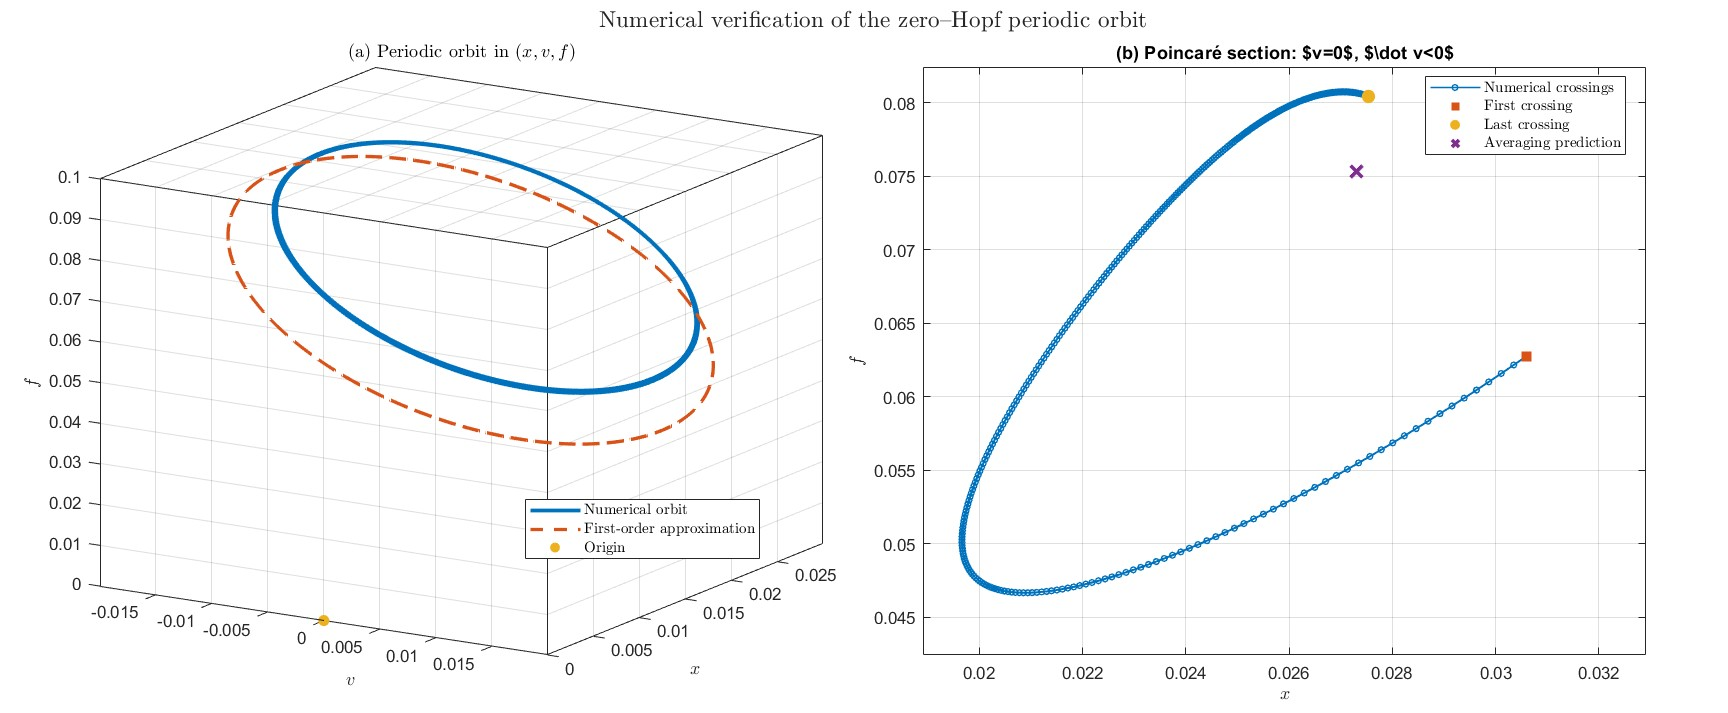
\includegraphics[width=\textwidth]{ZH}
\caption{Numerical verification of the periodic orbit bifurcating from
the zero--Hopf equilibrium for
\(\omega_0=2\), \(\tau=1\), \(\kappa=1\), \(d=0.2\),
\(g_1=-0.2\), \(k_1=1\), and \(\varepsilon=0.02\).
Panel~(a) compares the periodic orbit obtained by numerical integration
of the full oscillator--actuator system with its leading-order
approximation obtained by averaging. Panel~(b) shows successive
intersections of the numerical trajectory with the Poincaré section
\(v=0\), \(\dot v<0\). Their convergence toward a single point provides
numerical evidence for the orbital asymptotic stability predicted by
\(\varepsilon g_1<0\).}
\label{fig:numerical-verification}
\end{figure}

\begin{theorem}[Main result]
\label{thm:main}

Assume
\[
\omega_0>0,\qquad
\tau>0,\qquad
\kappa\neq0,\qquad
\omega_0\tau>1.
\]
For every
\[
\sigma\in\mathcal I_{\mathrm H}\setminus\{0\},
\]
the equilibrium
\[
E_0=(0,0,0)
\]
undergoes a codimension-one Hopf bifurcation along the curve
\[
g=g_{\mathrm H}(\sigma),\qquad
k_s=k_{s,\mathrm H}(\sigma).
\]

Moreover, under the unfolding
\[
g=g_{\mathrm H}(\sigma),\qquad
k_s
=
k_{s,\mathrm H}(\sigma)
+\eta_2\varepsilon^2
+\eta_3\varepsilon^3,
\]
a unique small-amplitude periodic orbit bifurcates from the equilibrium
whenever
\[
\sigma\eta_2<0.
\]

Its leading-order asymptotic expansion is
\[
\begin{aligned}
x(t,\varepsilon)
&=
\varepsilon R_{\mathrm H}^*
\cos\bigl(\Omega_{\mathrm H}t+\theta_0\bigr)
+
O(\varepsilon^2),
\\
v(t,\varepsilon)
&=
-\varepsilon
\Omega_{\mathrm H}
R_{\mathrm H}^*
\sin\bigl(\Omega_{\mathrm H}t+\theta_0\bigr)
+
O(\varepsilon^2),
\\
f(t,\varepsilon)
&=
\varepsilon
\frac{1-\sigma\tau}{\tau^2}
R_{\mathrm H}^*
\cos\bigl(\Omega_{\mathrm H}t+\theta_0\bigr)
\\
&\quad+
\varepsilon
\frac{\Omega_{\mathrm H}(1-\sigma\tau)}{\tau}
R_{\mathrm H}^*
\sin\bigl(\Omega_{\mathrm H}t+\theta_0\bigr)
+
O(\varepsilon^2),
\end{aligned}
\]
where \(R_{\mathrm H}^*\) is given explicitly in
Section~\ref{subsec:classical-Hopf-second-order-averaging}.
The period satisfies
\[
T_\varepsilon
=
\frac{2\pi}{\Omega_{\mathrm H}}
+
O(\varepsilon).
\]

Finally, the bifurcation is supercritical for
\(\sigma>0\) and subcritical for \(\sigma<0\).

\end{theorem}


\subsection{Real canonical coordinates at the zero--Hopf point}
\label{subsec:zero-Hopf-canonical-coordinates}

At the critical parameter values
\[
g=g_{\mathrm{ZH}}
=
d+\frac1\tau,
\qquad
k_s=k_{s,\mathrm{ZH}}
=
\omega_0^2,
\]
the Jacobian matrix at the origin is
\begin{equation}
\label{eq:A-zero-Hopf}
A_{\mathrm{ZH}}
=
\begin{pmatrix}
0&1&0\\[1mm]
-\omega_0^2&1/\tau&1\\[2mm]
\omega_0^2/\tau&0&-1/\tau
\end{pmatrix}.
\end{equation}

We seek a real nonsingular matrix \(P_{\mathrm{ZH}}\) satisfying
\begin{equation}
\label{eq:zero-Hopf-similarity-objective}
P_{\mathrm{ZH}}^{-1}
A_{\mathrm{ZH}}
P_{\mathrm{ZH}}
=
J_{\mathrm{ZH}},
\end{equation}
where
\begin{equation}
\label{eq:zero-Hopf-Jordan-form}
J_{\mathrm{ZH}}
=
\begin{pmatrix}
0&-\Omega_{\mathrm{ZH}}&0\\
\Omega_{\mathrm{ZH}}&0&0\\
0&0&0
\end{pmatrix}.
\end{equation}

Writing
\[
P_{\mathrm{ZH}}
=
\begin{pmatrix}
p_1&p_2&p_3
\end{pmatrix},
\]
its columns are chosen to satisfy
\begin{equation}
\label{eq:zero-Hopf-column-relations}
A_{\mathrm{ZH}}p_1
=
\Omega_{\mathrm{ZH}}p_2,
\qquad
A_{\mathrm{ZH}}p_2
=
-\Omega_{\mathrm{ZH}}p_1,
\qquad
A_{\mathrm{ZH}}p_3=0.
\end{equation}
A convenient choice is
\begin{equation}
\label{eq:P-zero-Hopf}
P_{\mathrm{ZH}}
=
\begin{pmatrix}
1&0&1/\omega_0^2\\[3mm]
0&-\Omega_{\mathrm{ZH}}&0\\[2mm]
1/\tau^2&
\Omega_{\mathrm{ZH}}/\tau&
1
\end{pmatrix}.
\end{equation}
Its determinant is
\begin{equation}
\label{eq:det-P-zero-Hopf}
\det P_{\mathrm{ZH}}
=
-\frac{
\Omega_{\mathrm{ZH}}^3
}{
\omega_0^2
}
\neq0.
\end{equation}
Thus \(P_{\mathrm{ZH}}\) is nonsingular.

We introduce the real zero--Hopf coordinates \((X,Y,Z)\) by
\begin{equation}
\label{eq:zero-Hopf-coordinate-transformation}
\begin{pmatrix}
x\\v\\f
\end{pmatrix}
=
P_{\mathrm{ZH}}
\begin{pmatrix}
X\\Y\\Z
\end{pmatrix}.
\end{equation}
Equivalently,
\begin{equation}
\label{eq:zero-Hopf-coordinate-transformation-explicit}
\begin{aligned}
x
&=
X+\frac{Z}{\omega_0^2},
\\[2mm]
v
&=
-\Omega_{\mathrm{ZH}}Y,
\\[2mm]
f
&=
\frac{X}{\tau^2}
+
\frac{\Omega_{\mathrm{ZH}}}{\tau}Y
+
Z.
\end{aligned}
\end{equation}

Under the unfolding \eqref{eq:zero-Hopf-unfolding}, system
\eqref{eq:model} becomes
\begin{equation}
\label{eq:zero-Hopf-XYZ-system}
\begin{aligned}
\dot X
={}&
-\Omega_{\mathrm{ZH}}Y
+
\varepsilon
\left[
\frac{g_1}{\Omega_{\mathrm{ZH}}\tau}Y
-
\frac{k_1}{\Omega_{\mathrm{ZH}}^2\tau}X
-
\frac{k_1}
{\Omega_{\mathrm{ZH}}^2\omega_0^2\tau}Z
\right]
\\
&+
\frac{\kappa}
{\Omega_{\mathrm{ZH}}^2\tau}X^2
+
\frac{2\kappa}
{\Omega_{\mathrm{ZH}}^2\omega_0^2\tau}XZ
+
\frac{\kappa}
{\Omega_{\mathrm{ZH}}^2\omega_0^4\tau}Z^2,
\\[2mm]
\dot Y
={}&
\Omega_{\mathrm{ZH}}X
+
\varepsilon g_1Y,
\\[2mm]
\dot Z
={}&
\varepsilon
\left[
-\frac{
g_1\omega_0^2
}{
\Omega_{\mathrm{ZH}}\tau
}Y
+
\frac{
k_1\omega_0^2
}{
\Omega_{\mathrm{ZH}}^2\tau
}X
+
\frac{k_1}
{\Omega_{\mathrm{ZH}}^2\tau}Z
\right]
\\
&-
\frac{
\kappa\omega_0^2
}{
\Omega_{\mathrm{ZH}}^2\tau
}X^2
-
\frac{
2\kappa
}{
\Omega_{\mathrm{ZH}}^2\tau
}XZ
-
\frac{
\kappa
}{
\Omega_{\mathrm{ZH}}^2\omega_0^2\tau
}Z^2.
\end{aligned}
\end{equation}

At \(\varepsilon=0\), the linear motion in the \((X,Y)\)-plane is a
harmonic rotation with angular frequency \(\Omega_{\mathrm{ZH}}\), while
\(Z\) is a neutral coordinate.

%%%%%%%%%%%%%%%%%%%%%%%%%%%%%%%%%%%%%%%%%%%%%%%%%%%%%%%%%%%%%%%%%%%%%%%%%%%%%%%
\subsection{Scaled polar formulation}
\label{subsec:zero-Hopf-polar}
%%%%%%%%%%%%%%%%%%%%%%%%%%%%%%%%%%%%%%%%%%%%%%%%%%%%%%%%%%%%%%%%%%%%%%%%%%%%%%%

We seek periodic solutions whose distance from \(E_0\) is
\(O(|\varepsilon|)\). Accordingly, introduce
\begin{equation}
\label{eq:zero-Hopf-polar-transformation}
X
=
\varepsilon r\cos\theta,
\qquad
Y
=
\varepsilon r\sin\theta,
\qquad
Z
=
\varepsilon u,
\end{equation}
where
\[
r\geq0,
\qquad
u\in\mathbb R,
\qquad
\theta\in\mathbb S^1.
\]

Define
\begin{equation}
\label{eq:zero-Hopf-H-definition}
\mathcal H(r,u,\theta)
=
r\cos\theta+\frac{u}{\omega_0^2}.
\end{equation}
Then the original displacement variable satisfies
\[
x=\varepsilon\mathcal H(r,u,\theta).
\]

After substituting \eqref{eq:zero-Hopf-polar-transformation} into
\eqref{eq:zero-Hopf-XYZ-system} and taking \(\theta\) as the new
independent variable, the system assumes the standard first-order
averaging form
\begin{equation}
\label{eq:zero-Hopf-standard-averaging-form}
\begin{aligned}
r'
&=
\varepsilon
F_{\mathrm{ZH},1}(\theta,r,u)
+
O(\varepsilon^2),
\\[2mm]
u'
&=
\varepsilon
F_{\mathrm{ZH},2}(\theta,r,u)
+
O(\varepsilon^2),
\end{aligned}
\end{equation}
where the prime denotes differentiation with respect to \(\theta\).

To simplify the notation, define
\begin{equation}
\label{eq:zero-Hopf-PQR}
\begin{aligned}
\mathcal P(r,u,\theta)
={}&
\frac{
g_1r\sin\theta
}{
\Omega_{\mathrm{ZH}}\tau
}
-
\frac{k_1}
{\Omega_{\mathrm{ZH}}^2\tau}
\mathcal H(r,u,\theta)
+
\frac{\kappa}
{\Omega_{\mathrm{ZH}}^2\tau}
\mathcal H^2(r,u,\theta),
\\[2mm]
\mathcal Q(r,u,\theta)
={}&
g_1r\sin\theta,
\\[2mm]
\mathcal R(r,u,\theta)
={}&
-\frac{
g_1\omega_0^2r\sin\theta
}{
\Omega_{\mathrm{ZH}}\tau
}
+
\frac{
k_1\omega_0^2
}{
\Omega_{\mathrm{ZH}}^2\tau
}
\mathcal H(r,u,\theta)
\\
&-
\frac{
\kappa\omega_0^2
}{
\Omega_{\mathrm{ZH}}^2\tau
}
\mathcal H^2(r,u,\theta).
\end{aligned}
\end{equation}
Then
\begin{equation}
\label{eq:zero-Hopf-F-components}
F_{\mathrm{ZH},1}
=
\frac{
\mathcal P\cos\theta+\mathcal Q\sin\theta
}{
\Omega_{\mathrm{ZH}}
},
\qquad
F_{\mathrm{ZH},2}
=
\frac{
\mathcal R
}{
\Omega_{\mathrm{ZH}}
}.
\end{equation}
The functions \(F_{\mathrm{ZH},1}\) and \(F_{\mathrm{ZH},2}\) are
\(2\pi\)-periodic with respect to \(\theta\).

%%%%%%%%%%%%%%%%%%%%%%%%%%%%%%%%%%%%%%%%%%%%%%%%%%%%%%%%%%%%%%%%%%%%%%%%%%%%%%%
\subsection{First-order averaging}
\label{subsec:zero-Hopf-first-order-averaging}
%%%%%%%%%%%%%%%%%%%%%%%%%%%%%%%%%%%%%%%%%%%%%%%%%%%%%%%%%%%%%%%%%%%%%%%%%%%%%%%

The first averaged function associated with
\eqref{eq:zero-Hopf-standard-averaging-form} is
\begin{equation}
\label{eq:zero-Hopf-first-averaged-definition}
\mathbf f_{\mathrm{ZH}}(r,u)
=
\begin{pmatrix}
f_{\mathrm{ZH},1}(r,u)\\[2mm]
f_{\mathrm{ZH},2}(r,u)
\end{pmatrix}
=
\int_0^{2\pi}
\begin{pmatrix}
F_{\mathrm{ZH},1}(\theta,r,u)\\[2mm]
F_{\mathrm{ZH},2}(\theta,r,u)
\end{pmatrix}
\,d\theta.
\end{equation}

Using \eqref{eq:zero-Hopf-PQR}, the integrands can be written explicitly
as
\begin{equation}
\label{eq:zero-Hopf-F1-expanded}
\begin{aligned}
F_{\mathrm{ZH},1}
={}&
\frac{
g_1r\sin\theta\cos\theta
}{
\Omega_{\mathrm{ZH}}^2\tau
}
+
\frac{
g_1r\sin^2\theta
}{
\Omega_{\mathrm{ZH}}
}
-
\frac{
k_1r\cos^2\theta
}{
\Omega_{\mathrm{ZH}}^3\tau
}
\\
&-
\frac{
k_1u\cos\theta
}{
\Omega_{\mathrm{ZH}}^3\tau\omega_0^2
}
+
\frac{
\kappa r^2\cos^3\theta
}{
\Omega_{\mathrm{ZH}}^3\tau
}
\\
&+
\frac{
2\kappa ru\cos^2\theta
}{
\Omega_{\mathrm{ZH}}^3\tau\omega_0^2
}
+
\frac{
\kappa u^2\cos\theta
}{
\Omega_{\mathrm{ZH}}^3\tau\omega_0^4
},
\end{aligned}
\end{equation}
and
\begin{equation}
\label{eq:zero-Hopf-F2-expanded}
\begin{aligned}
F_{\mathrm{ZH},2}
={}&
-\frac{
g_1\omega_0^2r\sin\theta
}{
\Omega_{\mathrm{ZH}}^2\tau
}
+
\frac{
k_1\omega_0^2r\cos\theta
}{
\Omega_{\mathrm{ZH}}^3\tau
}
+
\frac{k_1u}
{\Omega_{\mathrm{ZH}}^3\tau}
\\
&-
\frac{
\kappa\omega_0^2r^2\cos^2\theta
}{
\Omega_{\mathrm{ZH}}^3\tau
}
-
\frac{
2\kappa ru\cos\theta
}{
\Omega_{\mathrm{ZH}}^3\tau
}
-
\frac{
\kappa u^2
}{
\Omega_{\mathrm{ZH}}^3\tau\omega_0^2
}.
\end{aligned}
\end{equation}

Integrating over one complete period yields
\begin{equation}
\label{eq:zero-Hopf-averaged-first-component}
f_{\mathrm{ZH},1}(r,u)
=
\frac{\pi r}{\Omega_{\mathrm{ZH}}}
\left(
g_1
-
\frac{
k_1
}{
\Omega_{\mathrm{ZH}}^2\tau
}
+
\frac{
2\kappa u
}{
\Omega_{\mathrm{ZH}}^2\tau\omega_0^2
}
\right),
\end{equation}
and
\begin{equation}
\label{eq:zero-Hopf-averaged-second-component}
f_{\mathrm{ZH},2}(r,u)
=
\frac{\pi}
{\Omega_{\mathrm{ZH}}^3\tau}
\left(
2k_1u
-
\kappa\omega_0^2r^2
-
\frac{2\kappa u^2}{\omega_0^2}
\right).
\end{equation}
Therefore,
\begin{equation}
\label{eq:zero-Hopf-first-averaged-function}
\mathbf f_{\mathrm{ZH}}(r,u)
=
\begin{pmatrix}
\dfrac{\pi r}{\Omega_{\mathrm{ZH}}}
\left(
g_1
-
\dfrac{k_1}{\Omega_{\mathrm{ZH}}^2\tau}
+
\dfrac{
2\kappa u
}{
\Omega_{\mathrm{ZH}}^2\tau\omega_0^2
}
\right)
\\[6mm]
\dfrac{\pi}{\Omega_{\mathrm{ZH}}^3\tau}
\left(
2k_1u
-
\kappa\omega_0^2r^2
-
\dfrac{2\kappa u^2}{\omega_0^2}
\right)
\end{pmatrix}.
\end{equation}

In particular, \(\mathbf f_{\mathrm{ZH}}\) does not vanish identically.
Thus first-order averaging is sufficient to detect periodic solutions
bifurcating from the zero--Hopf equilibrium.

%%%%%%%%%%%%%%%%%%%%%%%%%%%%%%%%%%%%%%%%%%%%%%%%%%%%%%%%%%%%%%%%%%%%%%%%%%%%%%%
\subsection{Zeros of the averaged function}
\label{subsec:zero-Hopf-averaged-zeros}
%%%%%%%%%%%%%%%%%%%%%%%%%%%%%%%%%%%%%%%%%%%%%%%%%%%%%%%%%%%%%%%%%%%%%%%%%%%%%%%

We seek zeros
\[
\mathbf f_{\mathrm{ZH}}(r,u)=0,
\qquad
r>0.
\]
The condition \(r>0\) excludes the equilibrium and corresponds to a
genuine oscillatory solution.

Since \(r>0\), the equation
\[
f_{\mathrm{ZH},1}(r,u)=0
\]
is equivalent to
\[
g_1
-
\frac{k_1}{\Omega_{\mathrm{ZH}}^2\tau}
+
\frac{
2\kappa u
}{
\Omega_{\mathrm{ZH}}^2\tau\omega_0^2
}
=
0.
\]
Hence
\begin{equation}
\label{eq:zero-Hopf-u0}
u_0
=
\frac{\omega_0^2}{2\kappa}
\left(
k_1
-
g_1\Omega_{\mathrm{ZH}}^2\tau
\right).
\end{equation}

Substituting \eqref{eq:zero-Hopf-u0} into
\[
f_{\mathrm{ZH},2}(r,u)=0
\]
gives
\[
2k_1u_0
-
\kappa\omega_0^2r^2
-
\frac{2\kappa u_0^2}{\omega_0^2}
=
0.
\]
After simplification,
\begin{equation}
\label{eq:zero-Hopf-r0-square}
r_0^2
=
\frac{
k_1^2
-
g_1^2\Omega_{\mathrm{ZH}}^4\tau^2
}{
2\kappa^2
}.
\end{equation}
Therefore,
\begin{equation}
\label{eq:zero-Hopf-r0}
r_0
=
\sqrt{
\frac{
k_1^2
-
g_1^2\Omega_{\mathrm{ZH}}^4\tau^2
}{
2\kappa^2
}
}.
\end{equation}

A nontrivial real zero exists precisely when
\begin{equation}
\label{eq:zero-Hopf-existence-condition}
k_1^2
-
g_1^2\Omega_{\mathrm{ZH}}^4\tau^2
>0.
\end{equation}
Under this condition, the averaged function has the zero
\begin{equation}
\label{eq:zero-Hopf-averaged-zero}
(r_0,u_0)
=
\left(
\sqrt{
\frac{
k_1^2
-
g_1^2\Omega_{\mathrm{ZH}}^4\tau^2
}{
2\kappa^2
}
},
\;
\frac{\omega_0^2}{2\kappa}
\left(
k_1
-
g_1\Omega_{\mathrm{ZH}}^2\tau
\right)
\right).
\end{equation}

%%%%%%%%%%%%%%%%%%%%%%%%%%%%%%%%%%%%%%%%%%%%%%%%%%%%%%%%%%%%%%%%%%%%%%%%%%%%%%%
\subsection{Nondegeneracy of the averaged zero}
\label{subsec:zero-Hopf-nondegeneracy}
%%%%%%%%%%%%%%%%%%%%%%%%%%%%%%%%%%%%%%%%%%%%%%%%%%%%%%%%%%%%%%%%%%%%%%%%%%%%%%%

The Jacobian matrix of the averaged function at \((r_0,u_0)\) is
\begin{equation}
\label{eq:zero-Hopf-averaged-Jacobian}
D\mathbf f_{\mathrm{ZH}}(r_0,u_0)
=
\begin{pmatrix}
0
&
\dfrac{
2\pi\kappa r_0
}{
\Omega_{\mathrm{ZH}}^3\tau\omega_0^2
}
\\[5mm]
-\dfrac{
2\pi\kappa\omega_0^2r_0
}{
\Omega_{\mathrm{ZH}}^3\tau
}
&
\dfrac{
2\pi g_1
}{
\Omega_{\mathrm{ZH}}
}
\end{pmatrix}.
\end{equation}
Its determinant is
\begin{equation}
\label{eq:zero-Hopf-averaged-Jacobian-determinant}
\det D\mathbf f_{\mathrm{ZH}}(r_0,u_0)
=
\frac{
2\pi^2
\left(
k_1^2
-
g_1^2\Omega_{\mathrm{ZH}}^4\tau^2
\right)
}{
\Omega_{\mathrm{ZH}}^6\tau^2
}.
\end{equation}
Condition \eqref{eq:zero-Hopf-existence-condition} therefore implies
\[
\det D\mathbf f_{\mathrm{ZH}}(r_0,u_0)>0.
\]
Thus the zero \((r_0,u_0)\) is isolated and nondegenerate.

By the first-order averaging theorem, for all sufficiently small
\(|\varepsilon|>0\), system
\eqref{eq:zero-Hopf-standard-averaging-form} possesses a
\(2\pi\)-periodic solution satisfying
\begin{equation}
\label{eq:zero-Hopf-periodic-reduced}
(r(\theta,\varepsilon),u(\theta,\varepsilon))
=
(r_0,u_0)+O(\varepsilon).
\end{equation}
This solution corresponds to a periodic orbit of the original
oscillator--actuator system.

%%%%%%%%%%%%%%%%%%%%%%%%%%%%%%%%%%%%%%%%%%%%%%%%%%%%%%%%%%%%%%%%%%%%%%%%%%%%%%%
\subsection{Stability of the periodic orbit}
\label{subsec:zero-Hopf-stability}
%%%%%%%%%%%%%%%%%%%%%%%%%%%%%%%%%%%%%%%%%%%%%%%%%%%%%%%%%%%%%%%%%%%%%%%%%%%%%%%

The trace and determinant of the averaged Jacobian are
\begin{equation}
\label{eq:zero-Hopf-trace-determinant}
\operatorname{tr}
D\mathbf f_{\mathrm{ZH}}(r_0,u_0)
=
\frac{
2\pi g_1
}{
\Omega_{\mathrm{ZH}}
},
\end{equation}
and
\begin{equation}
\label{eq:zero-Hopf-determinant-repeated}
\det
D\mathbf f_{\mathrm{ZH}}(r_0,u_0)
=
\frac{
2\pi^2
\left(
k_1^2
-
g_1^2\Omega_{\mathrm{ZH}}^4\tau^2
\right)
}{
\Omega_{\mathrm{ZH}}^6\tau^2
}
>0.
\end{equation}
The corresponding eigenvalues are
\begin{equation}
\label{eq:zero-Hopf-averaged-eigenvalues}
\lambda_\pm^{\mathrm{av}}
=
\frac{
\pi g_1
}{
\Omega_{\mathrm{ZH}}
}
\pm
\frac{\pi}
{\Omega_{\mathrm{ZH}}^3\tau}
\sqrt{
3g_1^2
\Omega_{\mathrm{ZH}}^4\tau^2
-
2k_1^2
}.
\end{equation}

Since the determinant is positive, the two eigenvalues have real parts
with the same sign, determined by the trace. Therefore,
\[
\operatorname{Re}
\lambda_\pm^{\mathrm{av}}<0
\quad\Longleftrightarrow\quad
g_1<0,
\]
and
\[
\operatorname{Re}
\lambda_\pm^{\mathrm{av}}>0
\quad\Longleftrightarrow\quad
g_1>0.
\]

The nontrivial Floquet multipliers of the periodic orbit satisfy
\begin{equation}
\label{eq:zero-Hopf-Floquet-expansion}
\mu_j
=
1+
\varepsilon
\lambda_j^{\mathrm{av}}
+
O(\varepsilon^2),
\qquad
j=1,2.
\end{equation}
Consequently, the periodic orbit is orbitally asymptotically stable when
\[
\varepsilon g_1<0
\]
and unstable when
\[
\varepsilon g_1>0.
\]

%%%%%%%%%%%%%%%%%%%%%%%%%%%%%%%%%%%%%%%%%%%%%%%%%%%%%%%%%%%%%%%%%%%%%%%%%%%%%%%
\subsection{Approximation of the bifurcating periodic orbit}
\label{subsec:zero-Hopf-orbit-approximation}
%%%%%%%%%%%%%%%%%%%%%%%%%%%%%%%%%%%%%%%%%%%%%%%%%%%%%%%%%%%%%%%%%%%%%%%%%%%%%%%

Returning to the original time variable, one has
\[
\dot\theta
=
\Omega_{\mathrm{ZH}}
+
O(\varepsilon),
\]
and hence
\begin{equation}
\label{eq:zero-Hopf-theta-time}
\theta(t,\varepsilon)
=
\Omega_{\mathrm{ZH}}t+\theta_0
+
O(\varepsilon),
\end{equation}
where \(\theta_0\) is an arbitrary initial phase.

Moreover,
\[
r(t,\varepsilon)=r_0+O(\varepsilon),
\qquad
u(t,\varepsilon)=u_0+O(\varepsilon).
\]
Therefore,
\begin{equation}
\label{eq:zero-Hopf-period}
T_\varepsilon
=
\frac{
2\pi
}{
\Omega_{\mathrm{ZH}}
}
+
O(\varepsilon).
\end{equation}

In the zero--Hopf coordinates,
\begin{equation}
\label{eq:zero-Hopf-XYZ-periodic}
\begin{aligned}
X(t,\varepsilon)
&=
\varepsilon r_0
\cos\left(
\Omega_{\mathrm{ZH}}t+\theta_0
\right)
+
O(\varepsilon^2),
\\[2mm]
Y(t,\varepsilon)
&=
\varepsilon r_0
\sin\left(
\Omega_{\mathrm{ZH}}t+\theta_0
\right)
+
O(\varepsilon^2),
\\[2mm]
Z(t,\varepsilon)
&=
\varepsilon u_0
+
O(\varepsilon^2).
\end{aligned}
\end{equation}

Using
\eqref{eq:zero-Hopf-coordinate-transformation-explicit}, the periodic
orbit in the original variables is
\begin{equation}
\label{eq:zero-Hopf-original-periodic-orbit}
\begin{aligned}
x(t,\varepsilon)
={}&
\varepsilon
\left[
r_0
\cos\left(
\Omega_{\mathrm{ZH}}t+\theta_0
\right)
+
\frac{u_0}{\omega_0^2}
\right]
+
O(\varepsilon^2),
\\[2mm]
v(t,\varepsilon)
={}&
-\varepsilon
\Omega_{\mathrm{ZH}}r_0
\sin\left(
\Omega_{\mathrm{ZH}}t+\theta_0
\right)
+
O(\varepsilon^2),
\\[2mm]
f(t,\varepsilon)
={}&
\varepsilon
\left[
\frac{r_0}{\tau^2}
\cos\left(
\Omega_{\mathrm{ZH}}t+\theta_0
\right)
+
\frac{
\Omega_{\mathrm{ZH}}r_0
}{\tau}
\sin\left(
\Omega_{\mathrm{ZH}}t+\theta_0
\right)
+
u_0
\right]
+
O(\varepsilon^2).
\end{aligned}
\end{equation}

Substituting
\eqref{eq:zero-Hopf-u0} and
\eqref{eq:zero-Hopf-r0}, one obtains
\begin{equation}
\label{eq:zero-Hopf-explicit-periodic-orbit}
\begin{aligned}
x(t,\varepsilon)
={}&
\varepsilon
\sqrt{
\frac{
k_1^2
-
g_1^2\Omega_{\mathrm{ZH}}^4\tau^2
}{
2\kappa^2
}
}
\cos\left(
\Omega_{\mathrm{ZH}}t+\theta_0
\right)
\\
&+
\frac{\varepsilon}{2\kappa}
\left(
k_1
-
g_1\Omega_{\mathrm{ZH}}^2\tau
\right)
+
O(\varepsilon^2),
\\[3mm]
v(t,\varepsilon)
={}&
-\varepsilon\Omega_{\mathrm{ZH}}
\sqrt{
\frac{
k_1^2
-
g_1^2\Omega_{\mathrm{ZH}}^4\tau^2
}{
2\kappa^2
}
}
\sin\left(
\Omega_{\mathrm{ZH}}t+\theta_0
\right)
+
O(\varepsilon^2),
\\[3mm]
f(t,\varepsilon)
={}&
\frac{\varepsilon}{\tau^2}
\sqrt{
\frac{
k_1^2
-
g_1^2\Omega_{\mathrm{ZH}}^4\tau^2
}{
2\kappa^2
}
}
\cos\left(
\Omega_{\mathrm{ZH}}t+\theta_0
\right)
\\
&+
\frac{
\varepsilon\Omega_{\mathrm{ZH}}
}{\tau}
\sqrt{
\frac{
k_1^2
-
g_1^2\Omega_{\mathrm{ZH}}^4\tau^2
}{
2\kappa^2
}
}
\sin\left(
\Omega_{\mathrm{ZH}}t+\theta_0
\right)
\\
&+
\frac{
\varepsilon\omega_0^2
}{2\kappa}
\left(
k_1
-
g_1\Omega_{\mathrm{ZH}}^2\tau
\right)
+
O(\varepsilon^2).
\end{aligned}
\end{equation}

Therefore, whenever
\[
k_1^2
-
g_1^2\Omega_{\mathrm{ZH}}^4\tau^2
>0,
\]
a periodic orbit bifurcates from the zero--Hopf equilibrium. Its
amplitude is proportional to \(|\varepsilon|\), its leading angular
frequency is \(\Omega_{\mathrm{ZH}}\), and its leading period is
\(2\pi/\Omega_{\mathrm{ZH}}\). Its orbital stability is determined by
the sign of \(\varepsilon g_1\).

%%%%%%%%%%%%%%%%%%%%%%%%%%%%%%%%%%%%%%%%%%%%%%%%

\section{Classical Hopf bifurcation}
\label{sec:classical-Hopf}

We investigate the classical Hopf bifurcation of the equilibrium
$E_0=(0,0,0)$ of system~\eqref{eq:model}. Throughout this section,
we assume
\[
\omega_0>0,\qquad
\tau>0,\qquad
\kappa\neq0,\qquad
\omega_0\tau>1.
\]
In contrast with the zero--Hopf configuration considered previously,
the classical Hopf configuration consists of a simple pair of
nonzero purely imaginary eigenvalues and a nonzero real eigenvalue.
We first determine the spectral locus and verify transversality.
We then compute the nonlinear bifurcation coefficient through
second-order averaging and establish existence, local uniqueness,
and stability of the bifurcating periodic orbit.

%\subsection{The spectral Hopf locus}
%\label{subsec:classical-Hopf-locus}

The characteristic polynomial of the linearization at $E_0$ is
\begin{equation}
\label{eq:classical-characteristic-polynomial}
p(\lambda;g,k_s)
=
\lambda^3+a_1(g)\lambda^2+a_2(g)\lambda+a_3(k_s),
\end{equation}
where
\begin{equation}
\label{eq:classical-cubic-coefficients}
a_1(g)=d-g+\frac1\tau,\qquad
a_2(g)=\omega_0^2+\frac{d-g}{\tau},\qquad
a_3(k_s)=\frac{\omega_0^2-k_s}{\tau}.
\end{equation}

Suppose that $p$ has roots $\pm i\varpi$, with $\varpi>0$.
Substituting $\lambda=i\varpi$ into
\eqref{eq:classical-characteristic-polynomial} and separating real
and imaginary parts gives
\[
a_3-a_1\varpi^2=0,\qquad
\varpi(a_2-\varpi^2)=0.
\]
Consequently,
\[
\varpi^2=a_2>0,\qquad a_3=a_1a_2.
\]
Requiring the remaining real eigenvalue to be nonzero yields
\begin{equation}
\label{eq:classical-Hopf-locus-original}
\frac{\omega_0^2-k_s}{\tau}
=
\left(d-g+\frac1\tau\right)
\left(\omega_0^2+\frac{d-g}{\tau}\right),
\end{equation}
subject to
\begin{equation}
\label{eq:classical-Hopf-basic-conditions}
\omega_0^2+\frac{d-g}{\tau}>0,
\qquad
d-g+\frac1\tau\neq0.
\end{equation}
Under these conditions,
\begin{equation}
\label{eq:classical-Hopf-factorization-general}
p(\lambda;g,k_s)
=
\left(\lambda+d-g+\frac1\tau\right)
\left(\lambda^2+\omega_0^2+\frac{d-g}{\tau}\right).
\end{equation}
These relations determine the spectral Hopf locus. Nonlinear
nondegeneracy will be established below.

%\subsection{Parametrization and the zero--Hopf limit}
%\label{subsec:Hopf-parametrization}

Introduce
$
\sigma=d-g+\frac1\tau
$
and define
\begin{equation}
\label{eq:classical-Hopf-gain}
g_{\mathrm H}(\sigma)=d+\frac1\tau-\sigma.
\end{equation}
The corresponding oscillatory frequency is
\begin{equation}
\label{eq:classical-Hopf-frequency}
\Omega_{\mathrm H}(\sigma)
=
\sqrt{\omega_0^2-\frac1{\tau^2}+\frac{\sigma}{\tau}}
=
\sqrt{\Omega_{\mathrm{ZH}}^2+\frac{\sigma}{\tau}}.
\end{equation}
Its domain is
\begin{equation}
\label{eq:classical-Hopf-sigma-domain}
\mathcal I_{\mathrm H}
=
\left\{\sigma\in\mathbb R:
\Omega_{\mathrm H}^2(\sigma)>0\right\}
=
\left(-\tau\Omega_{\mathrm{ZH}}^2,\infty\right).
\end{equation}
For $\sigma\in\mathcal I_{\mathrm H}$, set
\begin{equation}
\label{eq:classical-Hopf-stiffness}
k_{s,\mathrm H}(\sigma)
=
\omega_0^2-\tau\sigma\Omega_{\mathrm H}^2(\sigma).
\end{equation}
At the following parameter values the coefficients in
\eqref{eq:classical-cubic-coefficients} satisfy
\[
a_1=\sigma,\qquad
a_2=\Omega_{\mathrm H}^2(\sigma),\qquad
a_3=\sigma\Omega_{\mathrm H}^2(\sigma).
\]
Substitution into
\eqref{eq:classical-characteristic-polynomial} gives the stated
factorization. Thus we have this proposition:

\begin{proposition}
\label{prop:classical-Hopf-spectral-parametrization}
At
$
g=g_{\mathrm H}(\sigma),
k_s=k_{s,\mathrm H}(\sigma)$ and 
 $\sigma\in\mathcal I_{\mathrm H},
$
the characteristic polynomial at $E_0$ factors as
\begin{equation}
\label{eq:classical-Hopf-factorization}
p_{\mathrm H}(\lambda;\sigma)
=
(\lambda+\sigma)
\left(\lambda^2+\Omega_{\mathrm H}^2(\sigma)\right).
\end{equation}
Hence its eigenvalues are
\begin{equation}
\label{eq:classical-Hopf-spectrum}
-\sigma,\qquad
\pm i\Omega_{\mathrm H}(\sigma).
\end{equation}
\end{proposition}
For $\sigma>0$, the noncritical direction is stable, whereas for
$\sigma<0$ it is unstable. At $\sigma=0$,
\[
g_{\mathrm H}(0)=d+\frac1\tau,\qquad
k_{s,\mathrm H}(0)=\omega_0^2,\qquad
\Omega_{\mathrm H}(0)=\Omega_{\mathrm{ZH}},
\]
and the spectrum becomes $0,\pm i\Omega_{\mathrm{ZH}}$.
Thus the zero--Hopf point is the limiting spectral configuration
on this parametrized curve.

The second equilibrium branch is
$
E_1=
\left(
\frac{k_s-\omega_0^2}{\kappa},
0,
\frac{\omega_0^2(k_s-\omega_0^2)}{\kappa}
\right).
$
Along the spectral Hopf locus,
$
E_{1,\mathrm H}(\sigma)
=
\left(
-\frac{\tau\sigma\Omega_{\mathrm H}^2(\sigma)}{\kappa},
0,
-\frac{\tau\sigma\omega_0^2\Omega_{\mathrm H}^2(\sigma)}{\kappa}
\right).
$
For every fixed $\sigma\in\mathcal I_{\mathrm H}\setminus\{0\}$,
this equilibrium is distinct from $E_0$. The two equilibria
coalesce as $\sigma\to0$. All local statements below concern
$E_0$ with $\sigma\neq0$ fixed.

\subsection{Transversality and the parameter unfolding}
\label{subsec:classical-Hopf-transversality}

Fix
$
\sigma\in\mathcal I_{\mathrm H}\setminus\{0\}$and
$
g=g_{\mathrm H}(\sigma),
$
and use $k_s$ as the bifurcation parameter. For the remainder
of the calculations, write
\begin{equation}
\label{eq:classical-frequency-short}
\Omega=\Omega_{\mathrm H}(\sigma),\qquad
D_\sigma=\Omega^2+\sigma^2>0.
\end{equation}

Let $\lambda(k_s)$ be the eigenvalue branch satisfying
$\lambda(k_{s,\mathrm H}(\sigma))=i\Omega$. Since this eigenvalue
is simple, implicit differentiation gives
\[
\lambda'(k_s)
=
-\frac{p_{k_s}}{p_\lambda}
=
\frac1{\tau p_\lambda}.
\]
At the critical parameter,
\[
p_\lambda(i\Omega)
=
-2\Omega^2+2i\sigma\Omega.
\]
Therefore,
\begin{equation}
\label{eq:classical-Hopf-transversality-derivative}
\left.
\frac{d}{dk_s}\operatorname{Re}\lambda(k_s)
\right|_{k_s=k_{s,\mathrm H}(\sigma)}
=
-\frac1{2\tau D_\sigma}
=: \beta_{\mathrm H}<0.
\end{equation}
In particular, the spectral crossing is transversal.
With
$
\mu=k_s-k_{s,\mathrm H}(\sigma),
$
the critical pair satisfies
\begin{equation}
\label{eq:classical-Hopf-real-part-expansion}
\operatorname{Re}\lambda
=
-\frac{\mu}{2\tau D_\sigma}+O(\mu^2).
\end{equation}
Thus the pair lies in the right half-plane for $\mu<0$ and
in the left half-plane for $\mu>0$, provided $|\mu|$ is
sufficiently small.

We consider the unfolding
\begin{equation}
\label{eq:classical-Hopf-small-parameter-unfolding}
g=g_{\mathrm H}(\sigma),\qquad
k_s=k_{s,\mathrm H}(\sigma)
+\eta_2\varepsilon^2+\eta_3\varepsilon^3,
\end{equation}
where $\eta_2,\eta_3\in\mathbb R$ are fixed. The scaling
$\mu=O(\varepsilon^2)$ is adapted to periodic orbits of
amplitude $O(|\varepsilon|)$.

The critical spectral configuration occurs at $\varepsilon=0$.
For nonzero $\varepsilon$, the equilibrium generally lies off
the Hopf locus. Indeed, under
\eqref{eq:classical-Hopf-small-parameter-unfolding},
\[
p(\lambda)
=
(\lambda+\sigma)(\lambda^2+\Omega^2)
-\frac{\eta_2\varepsilon^2+\eta_3\varepsilon^3}{\tau}.
\]
A nonzero purely imaginary root requires
$\eta_2\varepsilon^2+\eta_3\varepsilon^3=0$.
In particular, if $\eta_2\neq0$, no such root exists for
sufficiently small nonzero $\varepsilon$.

All estimates below are understood for fixed $\sigma\neq0$
and fixed remaining parameters. Their constants and the
admissible size of $|\varepsilon|$ may depend on these
parameters.

%\subsection{Real Jordan coordinates}
%\label{subsec:classical-Jordan}

\subsection{The first averaged function and transverse correction}
\label{subsec:classical-first-average}
At $\varepsilon=0$, the Jacobian at $E_0$ is
\begin{equation}
\label{eq:A-sigma}
A_\sigma=
\begin{pmatrix}
0&1&0\\
-\omega_0^2&\dfrac1\tau-\sigma&1\\
\dfrac{k_{s,\mathrm H}(\sigma)}{\tau}&0&-\dfrac1\tau
\end{pmatrix}.
\end{equation}
Define
\begin{equation}
\label{eq:abc-sigma}
a_\sigma=\frac{1-\sigma\tau}{\tau^2},\qquad
b_\sigma=\frac{\Omega(1-\sigma\tau)}{\tau},\qquad
c_\sigma=\omega_0^2+\frac{\sigma}{\tau},
\end{equation}
and
\begin{equation}
\label{eq:P-sigma}
P_\sigma=
\begin{pmatrix}
1&0&1\\
0&-\Omega&-\sigma\\
a_\sigma&b_\sigma&c_\sigma
\end{pmatrix}.
\end{equation}
Its columns satisfy
\[
A_\sigma p_1=\Omega p_2,\qquad
A_\sigma p_2=-\Omega p_1,\qquad
A_\sigma p_3=-\sigma p_3.
\]
Moreover,
\[
\det P_\sigma=-\Omega D_\sigma\neq0.
\]
Consequently,
\begin{equation}
\label{eq:Jordan-sigma}
P_\sigma^{-1}A_\sigma P_\sigma
=
\begin{pmatrix}
0&-\Omega&0\\
\Omega&0&0\\
0&0&-\sigma
\end{pmatrix}.
\end{equation}

Introduce $(X,Y,Z)$ by
\begin{equation}
\label{eq:classical-coordinate-change}
\begin{pmatrix}x\\v\\f\end{pmatrix}
=
P_\sigma
\begin{pmatrix}X\\Y\\Z\end{pmatrix}.
\end{equation}
Explicitly,
\begin{equation}
\label{eq:classical-coordinate-explicit}
x=X+Z,\qquad
v=-\Omega Y-\sigma Z,\qquad
f=a_\sigma X+b_\sigma Y+c_\sigma Z.
\end{equation}

Set
\begin{equation}
\label{eq:H-classical}
\mathcal H(X,Z,\varepsilon)
=
\frac{\eta_2\varepsilon^2+\eta_3\varepsilon^3}{\tau}(X+Z)
-\frac{\kappa}{\tau}(X+Z)^2.
\end{equation}
Since
\[
P_\sigma^{-1}
\begin{pmatrix}0\\0\\1\end{pmatrix}
=
\begin{pmatrix}
-1/D_\sigma\\
-\sigma/(\Omega D_\sigma)\\
1/D_\sigma
\end{pmatrix},
\]
the full transformed system is
\begin{equation}
\label{eq:classical-XYZ-system}
\begin{aligned}
\dot X&=-\Omega Y-\frac{\mathcal H}{D_\sigma},\\
\dot Y&=\Omega X-\frac{\sigma\mathcal H}{\Omega D_\sigma},\\
\dot Z&=-\sigma Z+\frac{\mathcal H}{D_\sigma}.
\end{aligned}
\end{equation}
%\subsection{Scaled cylindrical coordinates}
%\label{subsec:classical-polar}
For $\varepsilon\neq0$, introduce
\begin{equation}
\label{eq:classical-scaled-polar}
X=\varepsilon R\cos\theta,\qquad
Y=\varepsilon R\sin\theta,\qquad
Z=\varepsilon W.
\end{equation}
The analysis is carried out locally with $R$ in a compact
subinterval of $(0,\infty)$ and $W$ near zero. Thus the
division by $R$ below causes no singularity.

Define
\begin{equation}
\label{eq:S-classical}
S(\theta,R,W)=R\cos\theta+W
\end{equation}
and
\begin{equation}
\label{eq:AB-classical}
A(\theta)=
\frac{\Omega\cos\theta+\sigma\sin\theta}{\Omega D_\sigma},
\qquad
B(\theta)=
\frac{\Omega\sin\theta-\sigma\cos\theta}{\Omega D_\sigma}.
\end{equation}
Then
\[
\mathcal H
=
-\frac{\kappa\varepsilon^2}{\tau}S^2
+\frac{\eta_2\varepsilon^3}{\tau}S
+\frac{\eta_3\varepsilon^4}{\tau}S.
\]
Substitution into \eqref{eq:classical-XYZ-system} yields
\begin{equation}
\label{eq:classical-RthetaW-time}
\begin{aligned}
\dot R
&=
\frac{\kappa\varepsilon}{\tau}S^2A
-\frac{\eta_2\varepsilon^2}{\tau}SA
+O(|\varepsilon|^3),\\
\dot\theta
&=
\Omega-\frac{\kappa\varepsilon}{\tau R}S^2B
+\frac{\eta_2\varepsilon^2}{\tau R}SB
+O(|\varepsilon|^3),\\
\dot W
&=
-\sigma W-\frac{\kappa\varepsilon}{\tau D_\sigma}S^2
+\frac{\eta_2\varepsilon^2}{\tau D_\sigma}S
+O(|\varepsilon|^3).
\end{aligned}
\end{equation}
The remainders are smooth and uniform on the compact
neighborhoods under consideration.

Since $\dot\theta=\Omega+O(|\varepsilon|)$ and $\Omega>0$,
we have $\dot\theta>0$ for sufficiently small
$|\varepsilon|$. We may therefore use $\theta$ as the
independent variable. Write
\[
q_1=-\frac{\kappa}{\tau R}S^2B,\qquad
q_2=\frac{\eta_2}{\tau R}SB.
\]
Then
\[
\frac1{\dot\theta}
=
\frac1\Omega-\varepsilon\frac{q_1}{\Omega^2}
+\varepsilon^2
\left(\frac{q_1^2}{\Omega^3}-\frac{q_2}{\Omega^2}\right)
+O(|\varepsilon|^3).
\]

With a prime denoting differentiation with respect to
$\theta$, the resulting system is
\begin{equation}
\label{eq:classical-theta-system}
\begin{pmatrix}R\\W\end{pmatrix}'
=
F_0(\theta,R,W)
+\varepsilon F_1(\theta,R,W)
+\varepsilon^2F_2(\theta,R,W)
+O(|\varepsilon|^3),
\end{equation}
where
\begin{equation}
\label{eq:F0-classical}
F_0=
\begin{pmatrix}0\\-\sigma W/\Omega\end{pmatrix},
\end{equation}
and
\begin{equation}
\label{eq:F1-classical}
\begin{aligned}
F_{1,1}
&=\frac{\kappa S^2}{\tau\Omega}A,\\
F_{1,2}
&=-\frac{\kappa S^2}{\tau\Omega D_\sigma}
-\frac{\sigma\kappa WS^2}{\tau R\Omega^2}B.
\end{aligned}
\end{equation}
The second-order terms are
\begin{equation}
\label{eq:F2-classical}
\begin{aligned}
F_{2,1}
&=
-\frac{\eta_2 S}{\tau\Omega}A
+\frac{\kappa^2S^4}{\tau^2R\Omega^2}AB,\\
F_{2,2}
&=
\frac{\eta_2 S}{\tau\Omega D_\sigma}
-\frac{\kappa^2S^4}{\tau^2D_\sigma R\Omega^2}B\\
&\quad
-\frac{\sigma\kappa^2WS^4}{\tau^2R^2\Omega^3}B^2
+\frac{\sigma\eta_2WS}{\tau R\Omega^2}B.
\end{aligned}
\end{equation}
All these functions are $2\pi$-periodic in $\theta$.
The coefficient $\eta_3$ first contributes at order
$\varepsilon^3$ in \eqref{eq:classical-theta-system}.



At $\varepsilon=0$, system
\eqref{eq:classical-theta-system} reduces to
\[
R'=0,\qquad W'=-\frac{\sigma}{\Omega}W.
\]
Its solutions are
\[
R(\theta)=R_0,\qquad
W(\theta)=W_0e^{-\sigma\theta/\Omega}.
\]
Thus $W_0=0$ gives a one-dimensional family of
$2\pi$-periodic solutions. The transverse return multiplier is
$
m_\sigma=e^{-2\pi\sigma/\Omega}\neq1.
$
This nondegeneracy allows us to solve the transverse
periodicity condition locally.

On $W=0$,
\[
F_{1,1}(\theta,R_0,0)
=
\frac{\kappa R_0^2\cos^2\theta}
{\tau\Omega^2D_\sigma}
\left(\Omega\cos\theta+\sigma\sin\theta\right).
\]
Hence the first averaged radial function is
\begin{equation}
\label{eq:classical-first-average-vanishes}
f_{\mathrm H,1}(R_0)
=
\int_0^{2\pi}F_{1,1}(\theta,R_0,0)\,d\theta
=0.
\end{equation}
To compute the next radial contribution, fix the initial
radial coordinate $R(0)=R_0$ and write
\begin{equation}
\label{eq:classical-Hopf-first-correction-expansion}
\begin{aligned}
R(\theta)&=R_0+\varepsilon r_1(\theta;R_0)
+O(\varepsilon^2),\\
W(\theta)&=\varepsilon w_1(\theta;R_0)
+O(\varepsilon^2).
\end{aligned}
\end{equation}
We impose $r_1(0;R_0)=0$ and choose $w_1$ to be
$2\pi$-periodic.

The radial correction satisfies
$
r_1'=F_{1,1}(\theta,R_0,0).
$
Integration gives
\begin{equation}
\label{eq:classical-Hopf-r1-explicit}
\begin{aligned}
r_1(\theta;R_0)
=
\frac{\kappa R_0^2}{\tau\Omega^2D_\sigma}
\left[
\Omega\left(\sin\theta-\frac{\sin^3\theta}{3}\right)
+\frac{\sigma}{3}(1-\cos^3\theta)
\right].
\end{aligned}
\end{equation}
In particular,
$
r_1(2\pi;R_0)=r_1(0;R_0)=0.
$
The transverse correction satisfies
\begin{equation}
\label{eq:classical-Hopf-w1-equation}
w_1'+\frac{\sigma}{\Omega}w_1
=
-\frac{\kappa R_0^2}{\tau\Omega D_\sigma}\cos^2\theta.
\end{equation}
Since $\sigma\neq0$, its homogeneous equation has no
nonzero $2\pi$-periodic solution. Therefore its periodic
solution is unique. Using
$\cos^2\theta=(1+\cos2\theta)/2$, we obtain
\begin{equation}
\label{eq:classical-Hopf-w1-explicit}
\begin{aligned}
w_1(\theta;R_0)
={}&
-\frac{\kappa R_0^2}{2\tau\sigma D_\sigma}\\
&-\frac{\kappa R_0^2\sigma}
{2\tau D_\sigma(4\Omega^2+\sigma^2)}\cos2\theta\\
&-\frac{\kappa R_0^2\Omega}
{\tau D_\sigma(4\Omega^2+\sigma^2)}\sin2\theta.
\end{aligned}
\end{equation}
Define
\begin{equation}
\label{eq:classical-gamma}
\gamma_\sigma(R_0)
=
w_1(0;R_0)
=
-\frac{\kappa R_0^2(\sigma^2+2\Omega^2)}
{\tau\sigma D_\sigma(\sigma^2+4\Omega^2)}.
\end{equation}
The transverse periodicity condition therefore requires
\begin{equation}
\label{eq:classical-W-initial}
W(0)=\varepsilon\gamma_\sigma(R_0)+O(\varepsilon^2).
\end{equation}

\subsection{The second-order radial bifurcation function}
\label{subsec:classical-second-average}

The second-order radial displacement, after imposing
transverse periodicity, is determined by
\begin{equation}
\label{eq:classical-Hopf-second-order-formula}
\begin{aligned}
f_{\mathrm H,2}(R_0)
=
\int_0^{2\pi}
\Big[
F_{2,1}(\theta,R_0,0)
&+\partial_R F_{1,1}(\theta,R_0,0)
r_1(\theta;R_0)\\
&+\partial_W F_{1,1}(\theta,R_0,0)
w_1(\theta;R_0)
\Big]\,d\theta.
\end{aligned}
\end{equation}
We evaluate these three contributions separately.

First,
\[
F_{2,1}(\theta,R_0,0)
=
-\frac{\eta_2R_0\cos\theta}{\tau\Omega}A(\theta)
+\frac{\kappa^2R_0^3\cos^4\theta}
{\tau^2\Omega^2}A(\theta)B(\theta).
\]
The identities
\[
\int_0^{2\pi}\cos\theta\,A(\theta)\,d\theta
=\frac{\pi}{D_\sigma},
\]
and
\[
\int_0^{2\pi}
\cos^4\theta\,A(\theta)B(\theta)\,d\theta
=
-\frac{\pi\sigma}{2\Omega D_\sigma^2}
\]
give
\begin{equation}
\label{eq:classical-Hopf-direct-second-integral}
\int_0^{2\pi}F_{2,1}(\theta,R_0,0)\,d\theta
=
-\frac{\pi\eta_2R_0}{\tau\Omega D_\sigma}
-\frac{\pi\kappa^2\sigma R_0^3}
{2\tau^2\Omega^3D_\sigma^2}.
\end{equation}

Second, since
\[
\partial_R F_{1,1}(\theta,R_0,0)
=
\frac2{R_0}F_{1,1}(\theta,R_0,0)
=
\frac2{R_0}r_1'(\theta;R_0),
\]
we have
\begin{equation}
\label{eq:classical-Hopf-radial-correction-integral}
\begin{aligned}
\int_0^{2\pi}
\partial_R F_{1,1}(\theta,R_0,0)
r_1(\theta;R_0)\,d\theta
&=
\frac1{R_0}
\left[r_1(\theta;R_0)^2\right]_0^{2\pi}\\
&=0.
\end{aligned}
\end{equation}
Third,
\[
\partial_W F_{1,1}(\theta,R_0,0)
=
\frac{2\kappa R_0\cos\theta}
{\tau\Omega^2D_\sigma}
\left(\Omega\cos\theta+\sigma\sin\theta\right).
\]

we obtain
\begin{equation}
\label{eq:classical-Hopf-transverse-correction-integral}
\begin{aligned}
&\int_0^{2\pi}
\partial_W F_{1,1}(\theta,R_0,0)
w_1(\theta;R_0)\,d\theta\\
&\qquad=
-\frac{\pi\kappa^2R_0^3}
{\tau^2\Omega\sigma D_\sigma^2}
-\frac{3\pi\kappa^2\sigma R_0^3}
{2\tau^2\Omega D_\sigma^2(4\Omega^2+\sigma^2)}.
\end{aligned}
\end{equation}
Combining these expressions gives
\begin{equation}
\label{eq:classical-Hopf-second-bifurcation-function}
\begin{aligned}
f_{\mathrm H,2}(R_0)
={}&
-\frac{\pi\eta_2}{\tau\Omega D_\sigma}R_0\\
&-\frac{\pi\kappa^2(8\Omega^2+\sigma^2)}
{2\tau^2\Omega^3\sigma D_\sigma(4\Omega^2+\sigma^2)}
R_0^3.
\end{aligned}
\end{equation}
In simplifying the cubic term, we use
\[
\sigma^4+9\Omega^2\sigma^2+8\Omega^4
=
(\Omega^2+\sigma^2)(8\Omega^2+\sigma^2).
\]

Equivalently,
\begin{equation}
\label{eq:classical-Hopf-second-bifurcation-factorized}
f_{\mathrm H,2}(R_0)
=
-\frac{\pi R_0}{\tau\Omega D_\sigma}
\left[\eta_2+\mathcal C_{\mathrm H}(\sigma)R_0^2\right],
\end{equation}
where
\begin{equation}
\label{eq:classical-Hopf-cubic-coefficient}
\mathcal C_{\mathrm H}(\sigma)
=
\frac{\kappa^2(8\Omega^2+\sigma^2)}
{2\tau\Omega^2\sigma(4\Omega^2+\sigma^2)}.
\end{equation}

A positive zero exists precisely when
%\begin{equation}
%\label{eq:classical-Hopf-existence-condition}
$\sigma\eta_2<0.$
%\end{equation}
Under this condition, it is
\begin{equation}
\label{eq:classical-Hopf-amplitude}
R_{\mathrm H}^*
=
\sqrt{
-\frac{2\tau\Omega^2\sigma(4\Omega^2+\sigma^2)}
{\kappa^2(8\Omega^2+\sigma^2)}\,\eta_2
}.
\end{equation}
Differentiating
\eqref{eq:classical-Hopf-second-bifurcation-factorized},
and using
$\mathcal C_{\mathrm H}(\sigma)(R_{\mathrm H}^*)^2=-\eta_2$,
gives
\begin{equation}
\label{eq:classical-Hopf-simple-root}
f_{\mathrm H,2}'(R_{\mathrm H}^*)
=
\frac{2\pi\eta_2}{\tau\Omega D_\sigma}\neq0.
\end{equation}
Thus the positive zero is simple.

\subsection{Existence and local uniqueness}
\label{subsec:classical-Hopf-existence-proof}

We give the return-map argument underlying the preceding
averaging calculation. This also specifies the local
uniqueness statement.

Assume $\sigma\eta_2<0$ and choose a compact interval
$J\subset(0,\infty)$ whose interior contains
$R_{\mathrm H}^*$. For initial conditions near
$J\times\{0\}$, let
\[
\mathcal P_\varepsilon(R_0,W_0)
=
\left(
\mathcal P_\varepsilon^R(R_0,W_0),
\mathcal P_\varepsilon^W(R_0,W_0)
\right)
\]
be the return map from $\theta=0$ to $\theta=2\pi$.
The map is smooth in its arguments and in $\varepsilon$.
At $\varepsilon=0$,
\[
\mathcal P_0(R_0,W_0)
=
(R_0,m_\sigma W_0),
\qquad
m_\sigma=e^{-2\pi\sigma/\Omega}.
\]
Since $m_\sigma-1\neq0$, the implicit function theorem
applied to
$
\mathcal P_\varepsilon^W(R_0,W_0)-W_0=0
$
gives a unique smooth function
$
W_0=\psi(R_0,\varepsilon)
$
near $J\times\{0\}$, with
\begin{equation}
\label{eq:classical-Hopf-transverse-elimination}
\psi(R_0,\varepsilon)
=
\varepsilon\gamma_\sigma(R_0)+O(\varepsilon^2).
\end{equation}
Define the reduced radial displacement
$
\Phi(R_0,\varepsilon)
=
\mathcal P_\varepsilon^R
\bigl(R_0,\psi(R_0,\varepsilon)\bigr)-R_0.
$
The first-order term vanishes by
\eqref{eq:classical-first-average-vanishes}, while
\eqref{eq:classical-Hopf-second-order-formula} gives
\begin{equation}
\label{eq:classical-Hopf-reduced-displacement}
\Phi(R_0,\varepsilon)
=
\varepsilon^2f_{\mathrm H,2}(R_0)
+O(|\varepsilon|^3),
\end{equation}
with the corresponding expansion also valid after
differentiation with respect to $R_0$.

The quotient $\Phi(R_0,\varepsilon)/\varepsilon^2$ extends
smoothly to $\varepsilon=0$, where it equals
$f_{\mathrm H,2}(R_0)$. By
\eqref{eq:classical-Hopf-simple-root}, a second application
of the implicit function theorem gives a unique root
\[
R_0=R_\varepsilon
=
R_{\mathrm H}^*+O(|\varepsilon|)
\]
near $R_{\mathrm H}^*$.
Consequently,
\[
\left(R_\varepsilon,\psi(R_\varepsilon,\varepsilon)\right)
\]
is a fixed point of $\mathcal P_\varepsilon$ for every
sufficiently small nonzero $\varepsilon$.

Since $R_\varepsilon>0$ and $\dot\theta>0$, this fixed point
represents a nonconstant periodic orbit of the original
system. Its initial scaled coordinates satisfy
\begin{equation}
\label{eq:classical-Hopf-initial-data}
\begin{aligned}
R(0,\varepsilon)
&=R_{\mathrm H}^*+O(|\varepsilon|),\\
W(0,\varepsilon)
&=\varepsilon\gamma_\sigma(R_{\mathrm H}^*)
+O(\varepsilon^2).
\end{aligned}
\end{equation}
The return-map argument proves uniqueness near this
positive scaled radius.

To establish the usual local Hopf uniqueness statement,
consider the radial normal form on a local center
manifold. Normalize its amplitude $\rho$ so that
\[
\rho=\sqrt{X^2+Y^2}
+O(X^2+Y^2)
\]
at the critical parameter. To the required order, the
radial equation is
\begin{equation}
\label{eq:classical-Hopf-radial-normal-form}
\dot\rho
=
\beta_{\mathrm H}\mu\rho
+\ell_{\mathrm H}(\sigma)\rho^3
+O\left(\mu^2\rho+|\mu|\rho^3+\rho^5\right).
\end{equation}
The cubic coefficient is obtained from the cubic return
displacement by multiplying by $\Omega/(2\pi)$:
\begin{equation}
\label{eq:classical-Hopf-radial-cubic-coefficient}
\ell_{\mathrm H}(\sigma)
=
-\frac{\kappa^2(8\Omega^2+\sigma^2)}
{4\tau^2\Omega^2\sigma
(\Omega^2+\sigma^2)(4\Omega^2+\sigma^2)}.
\end{equation}
This expression refers to the stated amplitude
normalization and to the original time variable.

Since
$
\beta_{\mathrm H}=-\frac1{2\tau D_\sigma}\neq0$
and
$\ell_{\mathrm H}(\sigma)\neq0,
$
the Hopf bifurcation is nondegenerate. The nondegenerate
Hopf theorem therefore gives local uniqueness of the
bifurcating periodic orbit, up to time translation, in a
sufficiently small neighborhood of $E_0$. This neighborhood
is chosen for the fixed value of $\sigma$ and need not
remain uniform as $\sigma\to0$.

Finally,
\begin{equation}
\label{eq:classical-Hopf-criticality-sign}
\operatorname{sgn}\ell_{\mathrm H}(\sigma)
=
-\operatorname{sgn}\sigma.
\end{equation}
Thus the bifurcation is supercritical for $\sigma>0$
and subcritical for $\sigma<0$. Here criticality is
understood in the usual Hopf sense, with the real part
of the critical eigenvalues as the unfolding coordinate.

\subsection{Approximation of the periodic orbit}
\label{subsec:classical-Hopf-periodic-orbit}

Assume $\sigma\eta_2<0$. The periodic solution constructed
above satisfies
\begin{equation}
\label{eq:classical-Hopf-RW-leading}
R(\theta,\varepsilon)
=
R_{\mathrm H}^*+O(|\varepsilon|),
\qquad
W(\theta,\varepsilon)=O(|\varepsilon|),
\end{equation}
uniformly in $\theta$ over one period. Periodicity extends
these bounds to all $\theta$.

More precisely,
\[
W(\theta,\varepsilon)
=
\varepsilon w_1(\theta;R_{\mathrm H}^*)
+O(\varepsilon^2).
\]
Consequently,
\[
Z(\theta,\varepsilon)
=
\varepsilon^2w_1(\theta;R_{\mathrm H}^*)
+O(|\varepsilon|^3).
\]

Since $\dot\theta=\Omega+O(|\varepsilon|)$,
\begin{equation}
\label{eq:classical-Hopf-theta-time}
\theta(t,\varepsilon)
=
\Omega t+\theta_0+O(|\varepsilon|),
\end{equation}
uniformly for $t$ in bounded intervals. Returning to the
original variables through
\eqref{eq:classical-coordinate-explicit}, we obtain
\begin{equation}
\label{eq:classical-Hopf-original-periodic-orbit}
\begin{aligned}
x(t,\varepsilon)
&=
\varepsilon R_{\mathrm H}^*
\cos(\Omega t+\theta_0)
+O(\varepsilon^2),\\
v(t,\varepsilon)
&=
-\varepsilon\Omega R_{\mathrm H}^*
\sin(\Omega t+\theta_0)
+O(\varepsilon^2),\\
f(t,\varepsilon)
&=
\varepsilon\frac{1-\sigma\tau}{\tau^2}
R_{\mathrm H}^*\cos(\Omega t+\theta_0)\\
&\quad+
\varepsilon\frac{\Omega(1-\sigma\tau)}{\tau}
R_{\mathrm H}^*\sin(\Omega t+\theta_0)
+O(\varepsilon^2).
\end{aligned}
\end{equation}
All remainders in
\eqref{eq:classical-Hopf-original-periodic-orbit} are
uniform on bounded time intervals. No uniform-in-time
claim is made with the limiting frequency $\Omega$.

The period is
\[
T_\varepsilon
=
\int_0^{2\pi}
\frac{d\theta}
{\dot\theta(\theta,R(\theta,\varepsilon),
W(\theta,\varepsilon),\varepsilon)}.
\]
On the leading periodic solution,
\[
q_1(\theta,R_{\mathrm H}^*,0)
=
-\frac{\kappa R_{\mathrm H}^*}{\tau}
\cos^2\theta\,B(\theta).
\]
Its integral over a period vanishes, because both
$\cos^2\theta\sin\theta$ and $\cos^3\theta$ have zero
integral. Therefore,
\begin{equation}
\label{eq:classical-Hopf-period}
T_\varepsilon
=
\frac{2\pi}{\Omega}
+O(\varepsilon^2).
\end{equation}
In particular, the displacement amplitude is
$|\varepsilon|R_{\mathrm H}^*+O(\varepsilon^2)$,
and the leading oscillatory frequency is $\Omega$.

\subsection{Floquet exponents and orbital stability}
\label{subsec:classical-Hopf-stability}

At $\varepsilon=0$, the return-map multipliers are
$1$ and $m_\sigma=e^{-2\pi\sigma/\Omega}$.
They are distinct because $\sigma\neq0$.
Thus the multiplier near $1$ can be followed smoothly.
The reduced displacement calculation gives
\begin{equation}
\label{eq:classical-Hopf-radial-multiplier}
\mu_{\mathrm{rad}}
=
1+\varepsilon^2
f_{\mathrm H,2}'(R_{\mathrm H}^*)
+O(|\varepsilon|^3).
\end{equation}
Here the elimination of the transverse fixed-point
equation gives the same leading correction as the
eigenvalue near $1$ of the full return-map derivative:
the other unperturbed multiplier is separated from $1$.

Using
\eqref{eq:classical-Hopf-simple-root} and
\eqref{eq:classical-Hopf-period}, the radial Floquet
exponent in the original time variable is
\begin{equation}
\label{eq:classical-Hopf-radial-exponent}
\begin{aligned}
\Lambda_{\mathrm{rad}}
&=
\frac1{T_\varepsilon}\log\mu_{\mathrm{rad}}\\
&=
\frac{\eta_2}{\tau D_\sigma}\varepsilon^2
+O(|\varepsilon|^3).
\end{aligned}
\end{equation}
Hence the radial direction is attracting for $\eta_2<0$
and repelling for $\eta_2>0$.

An exact divergence identity determines the transverse
exponent more precisely. The divergence of the original
vector field is
$
\operatorname{div}F
=
g-d-\frac1\tau.
$
Along the unfolding
\eqref{eq:classical-Hopf-small-parameter-unfolding}, this
quantity is identically $-\sigma$.
Liouville's formula, together with the trivial Floquet
multiplier $1$ of an autonomous periodic orbit, gives
\begin{equation}
\label{eq:classical-Hopf-multiplier-product}
\mu_{\mathrm{rad}}\mu_{\mathrm{tr}}
=
e^{-\sigma T_\varepsilon}.
\end{equation}
Both nontrivial multipliers are positive for sufficiently
small $|\varepsilon|$, since their limits are $1$ and
$m_\sigma>0$. Taking real logarithms therefore yields
\begin{equation}
\label{eq:classical-Hopf-exponent-sum}
\Lambda_{\mathrm{rad}}+\Lambda_{\mathrm{tr}}
=
-\sigma.
\end{equation}
Consequently,
\begin{equation}
\label{eq:classical-Hopf-transverse-exponent}
\Lambda_{\mathrm{tr}}
=
-\sigma
-\frac{\eta_2}{\tau D_\sigma}\varepsilon^2
+O(|\varepsilon|^3).
\end{equation}

If $\sigma>0$, the existence condition requires
$\eta_2<0$. Both nontrivial exponents are then negative,
and the periodic orbit is orbitally asymptotically stable.

If $\sigma<0$, the existence condition requires
$\eta_2>0$. Both nontrivial exponents are then positive,
and the periodic orbit is repelling in the two directions
transverse to the flow.

These stability conclusions agree with the sign of the
cubic coefficient in
\eqref{eq:classical-Hopf-radial-cubic-coefficient}.

\begin{remark}[Lack of uniformity near the zero--Hopf point]
\label{rem:classical-Hopf-nonuniformity}
The preceding analysis is performed for fixed
$\sigma\neq0$. As $\sigma\to0$,
\[
m_\sigma-1=e^{-2\pi\sigma/\Omega}-1\longrightarrow0,
\]
so the transverse periodicity equation loses its
nondegeneracy. The factor $1/\sigma$ in
$\gamma_\sigma$ and in the cubic coefficient reflects
the same loss of a noncritical transverse direction.
Accordingly, neither the neighborhood of local uniqueness
nor the bounds on $|\varepsilon|$ are asserted to be
uniform as $\sigma\to0$. At $\sigma=0$, the
two-dimensional zero--Hopf averaged system must be used.
\end{remark}

%\subsection{Main classical Hopf theorem}
%\label{subsec:classical-Hopf-main-theorem}

\begin{theorem}[Main Classical Hopf bifurcation]
\label{subsec:classical-Hopf-main-theorem}
Consider system~\eqref{eq:model} and assume
\[
\omega_0>0,\qquad
\tau>0,\qquad
\kappa\neq0,\qquad
\omega_0\tau>1.
\]
Let
$
\mathcal I_{\mathrm H}
=
\left\{
\sigma\in\mathbb R:
\omega_0^2-\frac1{\tau^2}+\frac{\sigma}{\tau}>0
\right\}.
$
For each fixed
$\sigma\in\mathcal I_{\mathrm H}\setminus\{0\}$, define
\[
\Omega=\Omega_{\mathrm H}(\sigma)
=
\sqrt{\omega_0^2-\frac1{\tau^2}+\frac{\sigma}{\tau}},
\qquad
D_\sigma=\Omega^2+\sigma^2,
\]
and
\[
g_{\mathrm H}(\sigma)=d+\frac1\tau-\sigma,\qquad
k_{s,\mathrm H}(\sigma)
=
\omega_0^2-\tau\sigma\Omega^2.
\]

At
$
g=g_{\mathrm H}(\sigma)$ and 
$k_s=k_{s,\mathrm H}(\sigma),
$
the origin is a nondegenerate classical Hopf equilibrium
with eigenvalues $-\sigma,\pm i\Omega$.
With $g$ fixed and $k_s$ as the bifurcation parameter,
the crossing coefficient is
$
\beta_{\mathrm H}=-\frac1{2\tau D_\sigma},
$
and the cubic radial coefficient, in the amplitude
normalization specified above, is
\[
\ell_{\mathrm H}(\sigma)
=
-\frac{\kappa^2(8\Omega^2+\sigma^2)}
{4\tau^2\Omega^2\sigma D_\sigma(4\Omega^2+\sigma^2)}.
\]
Fix $\eta_2,\eta_3\in\mathbb R$ with $\sigma\eta_2<0$,
and consider
$
g=g_{\mathrm H}(\sigma)$ and 
$k_s=k_{s,\mathrm H}(\sigma)
+\eta_2\varepsilon^2+\eta_3\varepsilon^3.
$
Then there exists $\varepsilon_0>0$ such that, for
$0<|\varepsilon|<\varepsilon_0$, a nonconstant periodic
orbit bifurcates from the origin. It is locally unique,
up to time translation, among periodic orbits in a
sufficiently small neighborhood of the origin.

Its leading scaled amplitude is
\[
R_{\mathrm H}^*
=
\sqrt{
-\frac{2\tau\Omega^2\sigma(4\Omega^2+\sigma^2)}
{\kappa^2(8\Omega^2+\sigma^2)}\,\eta_2
},
\]
and its period satisfies
$
T_\varepsilon=\frac{2\pi}{\Omega}+O(\varepsilon^2).
$
For a suitable phase $\theta_0$, its components satisfy
\[
\begin{aligned}
x(t,\varepsilon)
&=
\varepsilon R_{\mathrm H}^*
\cos(\Omega t+\theta_0)+O(\varepsilon^2),\\
v(t,\varepsilon)
&=
-\varepsilon\Omega R_{\mathrm H}^*
\sin(\Omega t+\theta_0)+O(\varepsilon^2),\\
f(t,\varepsilon)
&=
\varepsilon\frac{1-\sigma\tau}{\tau^2}
R_{\mathrm H}^*\cos(\Omega t+\theta_0)\\
&\quad+
\varepsilon\frac{\Omega(1-\sigma\tau)}{\tau}
R_{\mathrm H}^*\sin(\Omega t+\theta_0)
+O(\varepsilon^2),
\end{aligned}
\]
uniformly for $t$ in bounded intervals.

The two nontrivial Floquet exponents satisfy
\[
\Lambda_{\mathrm{rad}}
=
\frac{\eta_2}{\tau D_\sigma}\varepsilon^2
+O(|\varepsilon|^3),
\]
and
\[
\Lambda_{\mathrm{tr}}
=
-\sigma
-\frac{\eta_2}{\tau D_\sigma}\varepsilon^2
+O(|\varepsilon|^3).
\]
Moreover, their sum is exactly $-\sigma$.

If $\sigma>0$, the Hopf bifurcation is supercritical
and the periodic orbit is orbitally asymptotically
stable. If $\sigma<0$, the bifurcation is subcritical
and the periodic orbit is repelling in both nontrivial
Floquet directions.

All neighborhood and smallness assertions are made for
fixed $\sigma\neq0$; no uniformity as $\sigma\to0$ is
asserted.
\end{theorem}

\begin{proof}
The spectral factorization follows from
Proposition~\ref{prop:classical-Hopf-spectral-parametrization}.
Equation~\eqref{eq:classical-Hopf-transversality-derivative}
establishes transversality. The second-order calculation
\eqref{eq:classical-Hopf-second-bifurcation-function}
gives the positive simple zero
\eqref{eq:classical-Hopf-amplitude} when
$\sigma\eta_2<0$.

The return-map construction in
Subsection~\ref{subsec:classical-Hopf-existence-proof}
then gives a periodic orbit for every sufficiently small
nonzero $\varepsilon$. The nonvanishing crossing and
cubic coefficients establish a nondegenerate Hopf
bifurcation and its local uniqueness up to time
translation.

The coordinate transformation and the estimates in
Subsection~\ref{subsec:classical-Hopf-periodic-orbit}
give the stated component expansions and period.
Finally,
\eqref{eq:classical-Hopf-radial-exponent} and
\eqref{eq:classical-Hopf-exponent-sum} give the Floquet
exponents. Their signs, together with
\eqref{eq:classical-Hopf-criticality-sign}, yield the
stability and criticality conclusions.
\end{proof}



\section{Dynamics at infinity}
\label{sec:infinity}

We study system~\eqref{eq:model} on the sphere at infinity using
the Poincar\'e compactification. We first examine the equations
in the local charts and then use these descriptions to determine
the connections between the equilibria on the sphere.
Throughout this section, assume $\omega_0>0$, $\tau>0$, and
$\kappa\neq0$, and write
\[
a=\omega_0^2,\qquad b=d-g,\qquad c=\frac{k_s}{\tau},
\qquad h=\frac1\tau,\qquad k=\frac{\kappa}{\tau}.
\]
Then the system becomes
\begin{equation}
\label{eq:abbreviated-infinity}
\dot x=v,\qquad
\dot v=-ax-bv+f,\qquad
\dot f=cx-hf-kx^2.
\end{equation}
Since $k\neq0$, this vector field has degree two.

\subsection{Compactification in the local charts}
\label{subsec:infinity-charts}

Let $U_1,U_2,U_3$ be the charts corresponding to the positive
$x$-, $v$-, and $f$-directions, and let $V_1,V_2,V_3$ be
their negative counterparts. In each chart, infinity is
represented by $w=0$, while $w>0$ corresponds to finite points.
We use the time change
\begin{equation}
\label{eq:chart-time}
\frac{dt}{ds}=w
\end{equation}
and denote differentiation with respect to $s$ by a prime.
The resulting polynomial equations represent the compactified
flow up to a positive smooth time factor in each chart.

In $U_1$, set
\[
u=\frac vx,\qquad q=\frac fx,\qquad w=\frac1x.
\]
The quotient rule gives
\[
\frac{du}{dt}=-a-bu+q-u^2,\qquad
\frac{dq}{dt}=c-hq-uq-\frac{k}{w},\qquad
\frac{dw}{dt}=-uw.
\]
After the time change~\eqref{eq:chart-time}, we obtain
\begin{equation}
\label{eq:chart-U1}
\begin{aligned}
u'&=w(-a-bu+q-u^2),\\
q'&=-k+w(c-hq-uq),\\
w'&=-uw^2.
\end{aligned}
\end{equation}
On $w=0$, this reduces to
\begin{equation}
\label{eq:boundary-U1}
u'=0,\qquad q'=-k.
\end{equation}
Thus there are no equilibria at infinity in $U_1$.

In $U_2$, take
\[
u=\frac xv,\qquad q=\frac fv,\qquad w=\frac1v,
\qquad L(u,q)=-au-b+q.
\]
The same calculation yields
\begin{equation}
\label{eq:chart-U2}
\begin{aligned}
u'&=w\bigl(1-uL(u,q)\bigr),\\
q'&=-ku^2+w\bigl(cu-hq-qL(u,q)\bigr),\\
w'&=-w^2L(u,q).
\end{aligned}
\end{equation}
Hence the equations at infinity are
\begin{equation}
\label{eq:boundary-U2}
u'=0,\qquad q'=-ku^2.
\end{equation}
Their equilibria form the line $u=0$.

Finally, in $U_3$, set
\[
u=\frac xf,\qquad q=\frac vf,\qquad w=\frac1f.
\]
The compactified equations are
\begin{equation}
\label{eq:chart-U3}
\begin{aligned}
u'&=ku^3+w(q-cu^2+hu),\\
q'&=ku^2q+w(-au-bq+1-cuq+hq),\\
w'&=ku^2w-w^2(cu-h).
\end{aligned}
\end{equation}
Their restriction to $w=0$ is
\begin{equation}
\label{eq:boundary-U3}
u'=ku^3,\qquad q'=ku^2q,
\end{equation}
whose equilibrium set is again the line $u=0$.

For the negative charts, use
\[
V_1:\ (x,v,f)=\frac{(-1,-u,-q)}w,\qquad
V_2:\ (x,v,f)=\frac{(-u,-1,-q)}w,\qquad
V_3:\ (x,v,f)=\frac{(-u,-q,-1)}w,
\]
with $w>0$ and the same time change. On $w=0$, we find
\begin{equation}
\label{eq:negative-boundary-charts}
\begin{aligned}
V_1:&\quad u'=0,\qquad q'=k,\\
V_2:&\quad u'=0,\qquad q'=ku^2,\\
V_3:&\quad u'=-ku^3,\qquad q'=-ku^2q.
\end{aligned}
\end{equation}
Thus the boundary equations in antipodal charts differ by a
change of sign. All local classifications below concern these
two-dimensional restrictions to $w=0$.

\subsection{The equilibrium set at infinity}
\label{subsec:infinity-equilibria}

Write
\[
S_\infty^2=\{(X,V,F)\in\mathbb R^3:X^2+V^2+F^2=1\},
\qquad p_f^\pm=(0,0,\pm1).
\]
Here $(X,V,F)$ represents a direction in the original phase
space, and $p_f^\pm$ are the force-axis endpoints.

The charts $U_1$ and $V_1$ cover all directions with $X\neq0$.
Neither contains an equilibrium at infinity. In $U_2$, the
line $u=0$ corresponds to
\[
(X,V,F)=\frac{(0,1,q)}{\sqrt{1+q^2}},\qquad q\in\mathbb R,
\]
which gives all directions with $X=0$ and $V>0$.
The chart $V_2$ gives the directions with $X=0$ and $V<0$.
The only remaining points with $X=0$ are $p_f^+$ and $p_f^-$;
they are equilibria at the origins of $U_3$ and $V_3$.
Therefore the complete equilibrium set is the great circle
\begin{equation}
\label{eq:equilibrium-circle}
\mathcal E_\infty=\{(X,V,F)\in S_\infty^2:X=0\}.
\end{equation}

The boundary Jacobians in $U_2$ and $U_3$ are, respectively,
\[
\begin{pmatrix}0&0\\-2ku&0\end{pmatrix},
\qquad
k\begin{pmatrix}3u^2&0\\2uq&u^2\end{pmatrix}.
\]
Both vanish on $u=0$, as do their counterparts in the negative
charts. Linearization therefore does not determine the local
behavior. Instead, we use the explicit solutions of the
boundary equations.

\subsection{Local phase portraits}
\label{subsec:infinity-local-portraits}

\paragraph{Points other than $p_f^\pm$.}
Every such point of $\mathcal E_\infty$ has $V\neq0$, so it
can be studied in $U_2$ or $V_2$. In $U_2$, let $(0,q_*)$
be the equilibrium under consideration and put $z=q-q_*$.
Then
\begin{equation}
\label{eq:infinity-generic-local}
u'=0,\qquad z'=-ku^2,
\end{equation}
with solutions
\begin{equation}
\label{eq:infinity-generic-solutions}
u(s)=u_0,\qquad z(s)=z_0-ku_0^2s.
\end{equation}
The line $u=0$ is stationary. On either side of it,
trajectories are straight lines parallel to the equilibrium
line, directed toward decreasing $z$ if $k>0$ and increasing
$z$ if $k<0$. Since $u$ remains a nonzero constant on every
moving trajectory, none approaches $(0,q_*)$ in either time
direction. The portrait in $V_2$ is the same with the arrows
reversed.

\paragraph{The force-axis endpoints.}
The point $p_f^+$ is the origin of $U_3$. In
\eqref{eq:boundary-U3}, points with $u=0$ are stationary.
For $u\neq0$, we have
\[
\frac{dq}{du}=\frac qu,
\]
so the nonstationary trajectories lie on the rays
\begin{equation}
\label{eq:infinity-ray-orbits}
q=Cu,\qquad C\in\mathbb R,\qquad u\neq0.
\end{equation}
Indeed, the solution through $(u_0,q_0)$, with $u_0\neq0$, is
\begin{equation}
\label{eq:infinity-U3-explicit}
(u(s),q(s))=
\frac{(u_0,q_0)}{\sqrt{1-2ku_0^2s}},
\qquad 1-2ku_0^2s>0.
\end{equation}
For $k>0$, it approaches the origin as $s\to-\infty$ and
moves away in forward time. Thus the rays at $p_f^+$ are
outgoing.

At $p_f^-$, the boundary equations in $V_3$ have the opposite
sign, and their solutions are
\begin{equation}
\label{eq:infinity-V3-explicit}
(u(s),q(s))=
\frac{(u_0,q_0)}{\sqrt{1+2ku_0^2s}},
\qquad 1+2ku_0^2s>0.
\end{equation}
For $k>0$, these rays approach the origin as $s\to+\infty$.
They are therefore incoming at $p_f^-$. When $k<0$, both
orientations reverse. Any divergence of these chart coordinates
only marks departure from the chart, not termination of the
global compactified orbit.

To determine stability on the sphere, put $r^2=u^2+q^2$.
Then
\begin{equation}
\label{eq:infinity-local-radius}
(r^2)'=
\begin{cases}
2ku^2r^2,&\text{in }U_3,\\
-2ku^2r^2,&\text{in }V_3.
\end{cases}
\end{equation}
At the endpoint with incoming rays, $r$ cannot increase in
forward time. This proves Lyapunov stability. The endpoint is
not asymptotically stable, however, because every neighborhood
contains other equilibria on $u=0$, and these points remain
fixed rather than converge to the endpoint. At the opposite
endpoint, arbitrarily close nonstationary points move away,
giving forward instability and Lyapunov stability in reversed
time. These are nonisolated equilibria, not isolated nodes
or cusps.

\begin{figure}[htbp]
\centering
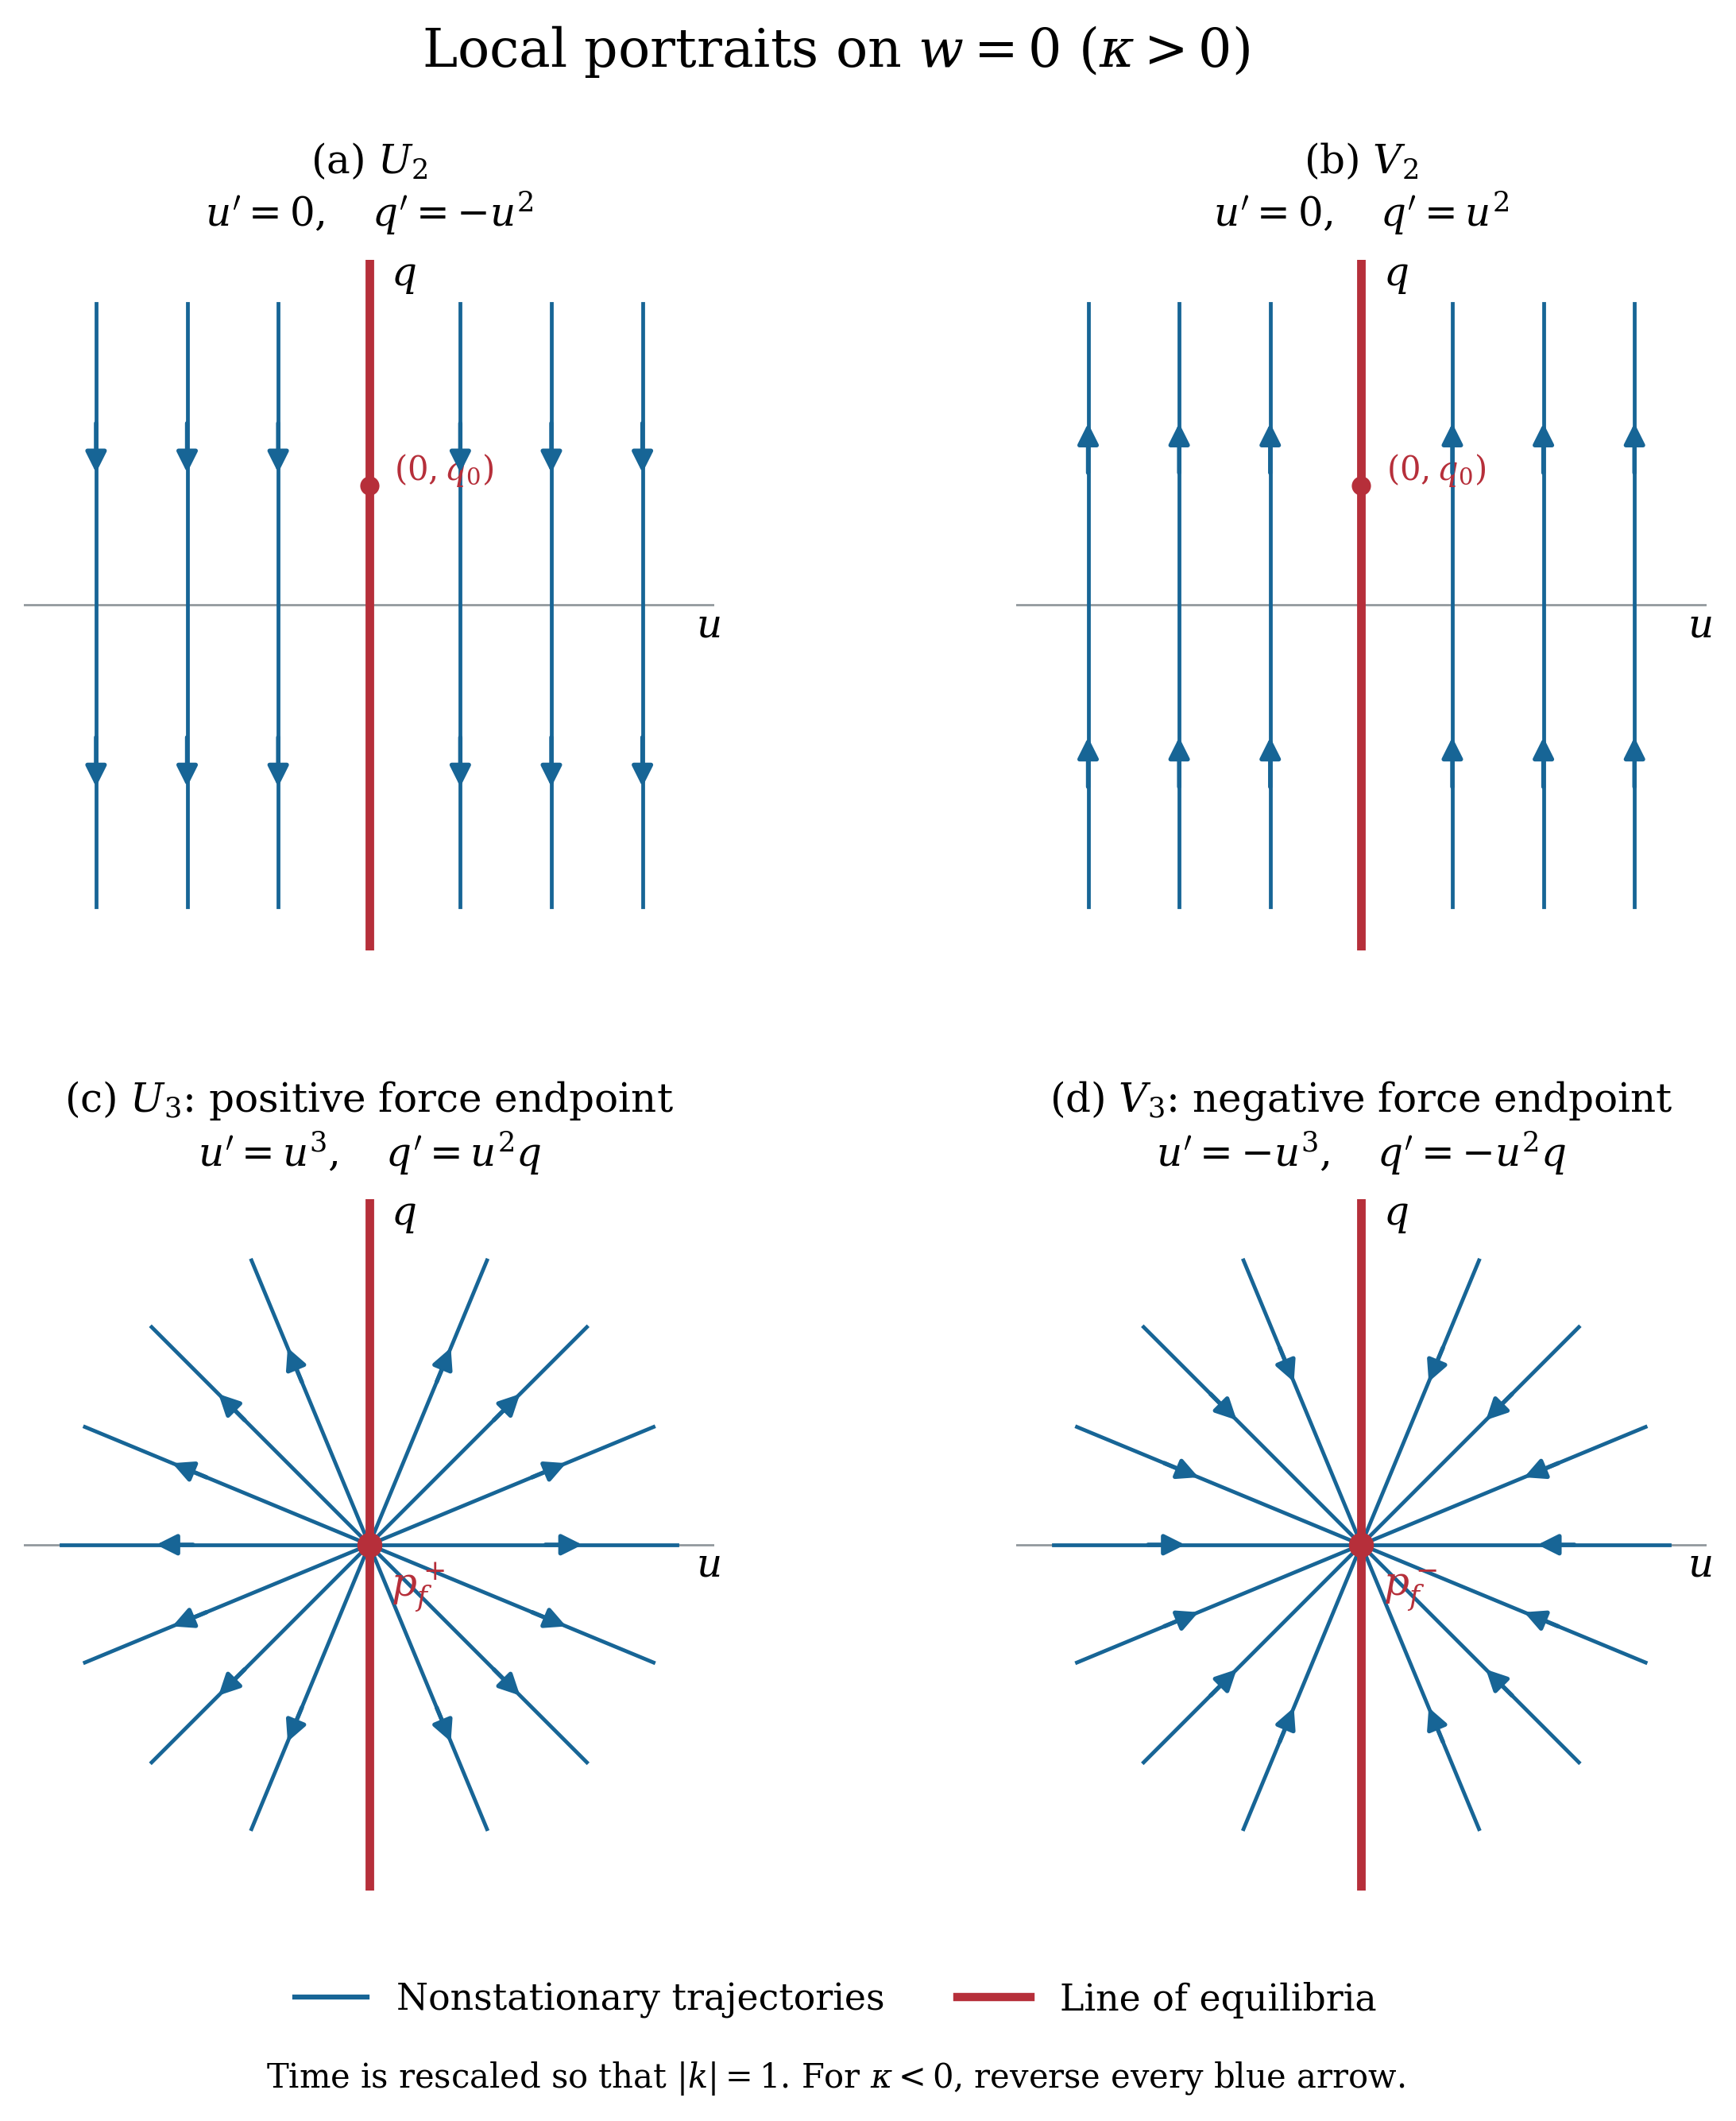
\includegraphics[width=\textwidth]{local}
\caption{Local boundary portraits for $\kappa>0$, after
a positive time rescaling setting $k=1$. In $U_2$ and $V_2$,
moving trajectories run parallel to the red equilibrium line.
In $U_3$ and $V_3$, they form outgoing and incoming rays at
$p_f^+$ and $p_f^-$, respectively. Every point on a red line
is stationary. For $\kappa<0$, all blue arrows reverse.}
\label{fig:local-infinity}
\end{figure}

\subsection{Global connections on the sphere at infinity}
\label{subsec:infinity-global-connections}

We now determine how these local trajectories connect on the
sphere. Every nonstationary point has $X\neq0$ and hence lies
in $U_1$ or $V_1$. First consider $U_1$. By
\eqref{eq:boundary-U1}, $u=m$ is constant and $q'= -k$.
On the sphere, this trajectory is represented by
\[
(X,V,F)=\frac{(1,m,q)}{\sqrt{1+m^2+q^2}},
\qquad q\in\mathbb R.
\]
It lies in the plane $V=mX$. This plane passes through the
center of the sphere and the force axis, so its intersection
with the sphere is a great circle. The condition $X>0$
selects one open semicircle. The other semicircle, with
$X<0$, is represented in $V_1$.

Thus all nonstationary orbits can be written as
\begin{equation}
\label{eq:great-semicircle-orbits}
\Gamma_{\delta,m}
=\left\{
\frac{\delta(1,m,q)}{\sqrt{1+m^2+q^2}}:q\in\mathbb R
\right\},
\qquad \delta\in\{-1,1\},\quad m\in\mathbb R.
\end{equation}
Their endpoints are determined by
\begin{equation}
\label{eq:chart-orbit-endpoints}
\lim_{q\to+\infty}
\frac{\delta(1,m,q)}{\sqrt{1+m^2+q^2}}=(0,0,\delta),
\qquad
\lim_{q\to-\infty}
\frac{\delta(1,m,q)}{\sqrt{1+m^2+q^2}}=(0,0,-\delta).
\end{equation}
Hence every nonstationary orbit joins $p_f^+$ and $p_f^-$.

If $k>0$, then $q$ decreases in $U_1$, giving the direction
from $p_f^+$ to $p_f^-$. In $V_1$, $q$ increases, but the
minus sign in the sphere representation gives the same
direction. Therefore
\begin{equation}
\label{eq:infinity-global-limits-positive}
\alpha(\Gamma_{\delta,m})=\{p_f^+\},\qquad
\omega(\Gamma_{\delta,m})=\{p_f^-\}
\qquad (k>0).
\end{equation}
For $k<0$, the arrows reverse, and
\begin{equation}
\label{eq:infinity-global-limits-negative}
\alpha(\Gamma_{\delta,m})=\{p_f^-\},\qquad
\omega(\Gamma_{\delta,m})=\{p_f^+\}.
\end{equation}
These limits are taken in the global compactified flow.
The chart time changes preserve orientation, and the smooth
flow on the compact sphere is complete. Its nonstationary
orbits approach the equilibrium endpoints only in infinite
compactified time.

Thus the outgoing rays at one endpoint continue along great
semicircles and become incoming rays at the other. Every
nonstationary boundary orbit is heteroclinic; no such orbit
is periodic or homoclinic. All boundary equations depend
only on $k$, whose magnitude changes the speed and whose
sign determines the orientation. Since $\tau>0$, the oriented
portrait depends only on the sign of $\kappa$.

\begin{figure}[htbp]
\centering
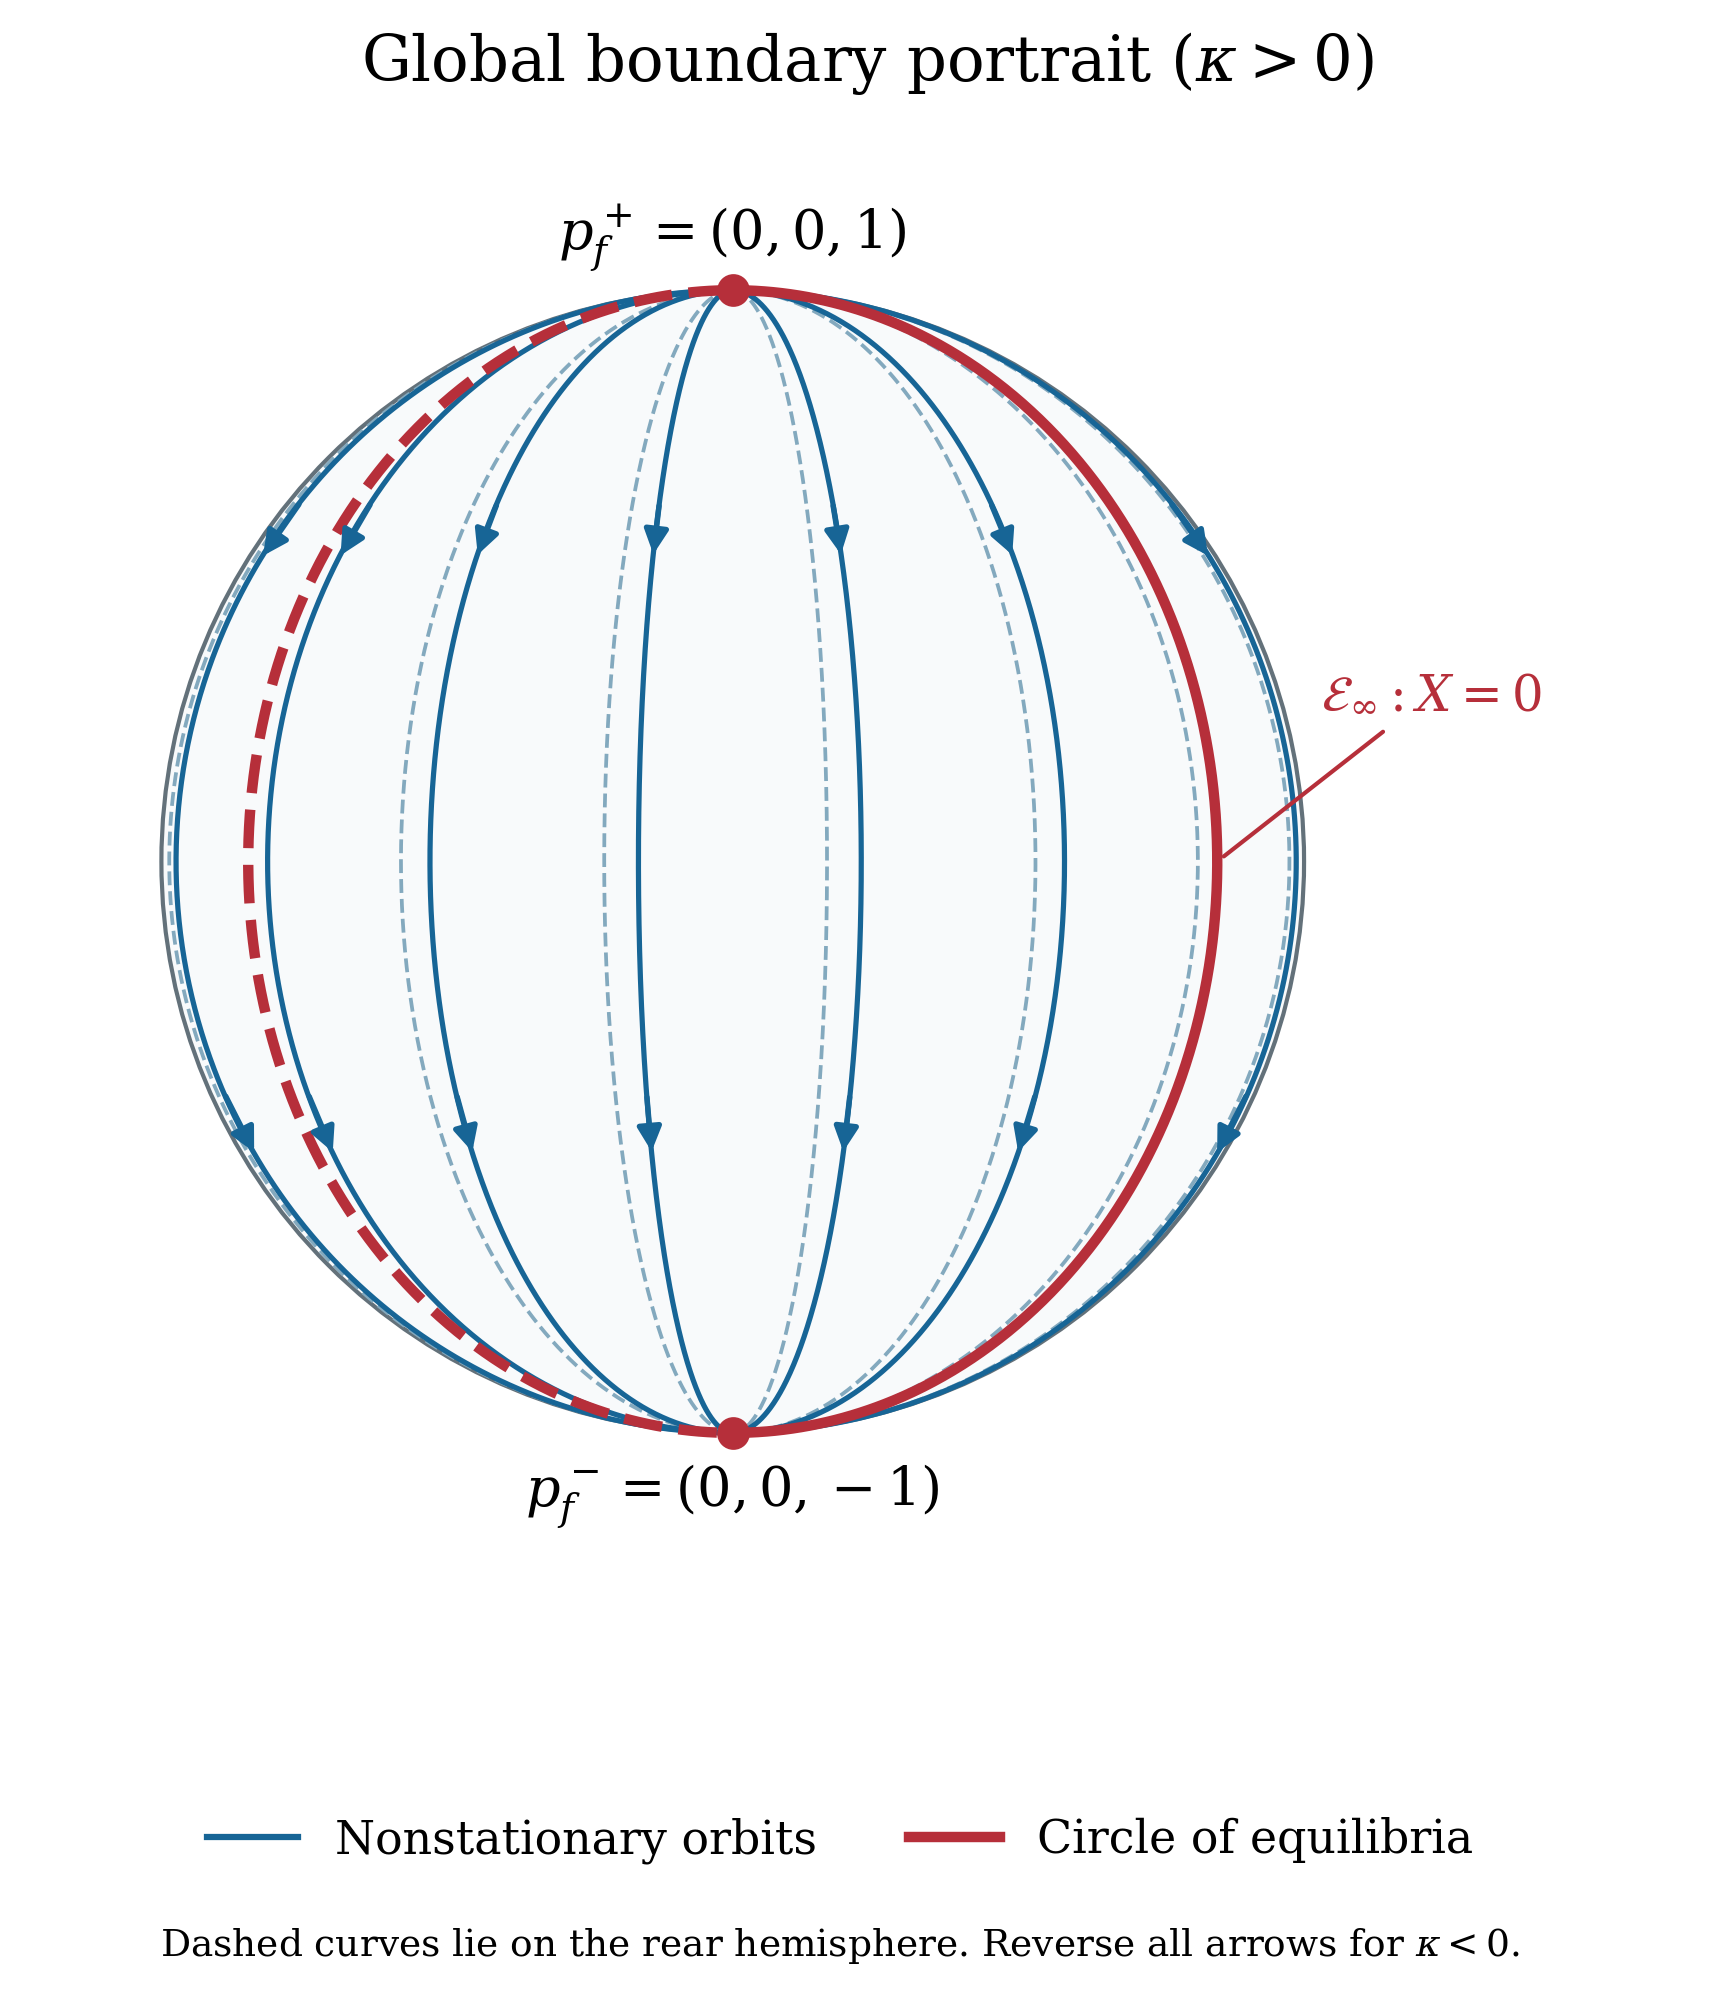
\includegraphics[width=0.58\textwidth]{global}
\caption{Boundary phase portrait for $\kappa>0$. The red
great circle $\mathcal E_\infty$ consists of equilibria.
Every nonstationary orbit is a great semicircle directed
from $p_f^+$ to $p_f^-$. Dashed curves lie on the rear
hemisphere. For $\kappa<0$, all arrows reverse.}
\label{fig:global-infinity}
\end{figure}

The preceding calculations establish the following result.

\begin{theorem}[Dynamics on the sphere at infinity]
\label{thm:dynamics-at-infinity}
Consider system~\eqref{eq:model} with $\omega_0>0$,
$\tau>0$, and $\kappa\neq0$. Its degree-two Poincar\'e
compactification has the following boundary dynamics.
\begin{enumerate}
\item
The equilibrium set is the great circle
$\mathcal E_\infty=\{X=0\}\cap S_\infty^2$, and the
boundary linearization vanishes at every equilibrium.
Away from $p_f^\pm$, the local portrait consists of an
equilibrium line with parallel moving trajectories on
both sides. At $p_f^\pm$, it consists of an equilibrium
line and incoming or outgoing rays in the force charts.
\item
Every nonstationary orbit is a great semicircle
\eqref{eq:great-semicircle-orbits}, directed from $p_f^+$
to $p_f^-$ if $\kappa>0$, and oppositely if $\kappa<0$.
There are no nonconstant periodic or homoclinic boundary
orbits.
\item
The common forward-limit endpoint is Lyapunov stable
but not asymptotically stable on the sphere. The other
endpoint is unstable forward in time and Lyapunov stable
in reversed time. The oriented boundary portrait depends
only on $\operatorname{sgn}\kappa$.
\end{enumerate}
\end{theorem}















\bibliographystyle{plain}
\bibliography{bibliography}


\end{document}